% !TeX root = RJwrapper.tex
\title{\pkg{exPrior}: An R Package for the Formulation of Ex-Situ Priors}
\author{by Falk He{\ss}e, Karina Cucchi, Nura Kawa, and Yoram Rubin}

\maketitle

\abstract{
The \CRANpkg{exPrior} package implements a procedure for formulating informative priors of geostatistical properties for a target field site, called \textit{ex-situ priors} and introduced in \cite{Cucchi2019}. 
The procedure uses a Bayesian hierarchical model to assimilate multiple types of data coming from multiple sites considered as similar to the target site. 
This prior summarizes the information contained in the data in the form of a probability density function that can be used to better inform further geostatistical investigations at the site.
The formulation of the prior uses ex-situ data, where the data set can either be gathered by the user or come in the form of a structured database. 
The package is designed to be flexible in that regard. 
For illustration purposes and for easiness of use, the package is ready to be used with the worldwide hydrogeological parameter database (WWHYPDA) \cite{Comunian2009}.
}

\section{Introduction}\label{sec:Introduction}

Characterizing the subsurface of our planet is an important task in fields such as geology, hydrogeology, and soil sciences. Yet compared to many other fields, the characterization of the subsurface is always burdened by large uncertainties. 
These uncertainties are caused by the general lack of data and the large spatial variability of many subsurface properties. 
The need to represent this uncertainty has led to the development of the field of geostatistics, wherein parameter values are treated as random variables defined by their probability distribution function (PDF). 
Today, the field of geostatistics has reached a mature state with many textbooks on the topic \citep{Pyrcz2002, Rubin2003, Kitanidis2008} and a solid number of software tools being available for practitioners (for an overview, see, e.g. \citet{Rubin2018}). 
For the R language \citep{R2014}, a solid ecosystem for geostatistical analysis has evolved in the last years \citep{Slater2019}. 
Packages like \CRANpkg{geoR} \citep{Ribeiro2001}, \CRANpkg{gstat} \citep{Pebesma2004}, \CRANpkg{georob} \citep{georob}, and \pkg{RGeostats} \citep{rgeostats_software} provide a large collection of tools for geostatistical analysis. Moreover, geostatistical databases can be conveniently accessed with packages like \CRANpkg{aqp} \citep{Beaudette2013} and textbooks on geostatistics are starting to provide all their examples in R code \citep{Diggle2007, Banerjee2014}.

Bayesian statistics provides the most appropriate framework to characterize uncertainty in general \citep{Hesse2019}. 
Bayesian methods are able to combine and assimilate data from disparate sources and jointly represent the different forms of uncertainty. 
As a result, Bayesian methods are nowadays increasingly employed in geostatistics and software implementations come as either standalone versions \citep{Vrugt2009-b, Rubin2010} or R packages like \CRANpkg{spBayes} \citep{Finley2015}, \pkg{R-INLA} \citep{Lindgren2015}, \CRANpkg{spTimer} \citep{Bakar2015}, \CRANpkg{BayesNSGP} \citep{Risser2020}, and \CRANpkg{anchoredDistr} \citep{Savoy2017-b}. 

Yet, there is no package to date, which would provide such tools with the necessary foundation, i.e. prior distributions for the modeled quantities. 
Since the prior is the first step of any Bayesian analysis, its overall importance can hardly be overstated. 
Moreover, the ability of prior distributions to represent available background information in a given field makes them an important source of information that should not be neglected. 
Integrating them into a Bayesian workflow should be straightforward since most packages for Bayesian inference allow users to specify their prior distributions.
%Given the aforementioned data scarcity, the ongoing disregard of this source therefore further exacerbates the already pressing problem of subsurface uncertainty. 
In addition, the use of informative prior distributions in this field is easy to motivate.
First, the parameters of geostatistical models are typically not simple convenience parameters but are part of physically-based partial differential equations. 
As a result, they correspond to real-world, physical measurements, making it possible to calibrate their prior distributions against empirical frequencies. 
Second, geostatistical models are usually site specific, making it conceptually easy to discriminate between the case-specific data, which should be used to compute the likelihood, and background data, which could be used to compute the prior distribution. 
In geostatistics, they are often called in-situ and ex-situ data, respectively.
Calibrating the prior against ex-situ data only, therefore guarantees a clear separation between likelihood and prior.

To provide practitioners therefore with a tool for prior derivation, this paper introduces the R package \CRANpkg{exPrior} \citep{exPrior_zenodo}. 
It implements the derivation of ex-situ priors, i.e., statistical distributions of subsurface properties at a given site from ex-situ data collected at similar sites, following the Bayesian hierarchical model developed by \citet{Cucchi2019}. 
The implementation is based on the \CRANpkg{nimble} package \citep{Valpine2017} itself based on the BUGS language \citep{Lunn2009}. 
The objective of the \CRANpkg{exPrior} package is to provide a ready-to-use software tool for assimilating ex-situ data into ex-situ priors. 
This will encourage the use of informative distributions for practitioners in geosciences that might not be experts in Bayesian hierarchical models and may find it therefore difficult to work with them otherwise. 
The focus of this package is on the Gaussian process (GP) modelling paradigm.
Although criticism exists, it is by far the most widely used paradigm, and a wide range range of software tools exist for the modeling of GPs \citep{Pebesma2004}.
Functions in \CRANpkg{exPrior} provide wrappers around \CRANpkg{nimble} functions implementing the Bayesian data assimilation framework. 
Non-expert practitioners can therefore apply this method without needing to implement the model itself. 
Moreover, the package is tightly integrated with two other R packages that help to expand its functionality.
First, the \pkg{geostatDB} package \citep{geostatDB_zenodo} provides access to a large data set from the worldwide hydrogeological parameter database (WWHYPDA) \cite{Comunian2009}.
Second, the \pkg{siteSimilarity} package \citep{siteSimilarity_zenodo} allows for clustering of similar sites and therefore facilitates a further reduction of uncertainty. 

Due to the background of the authors, the examples and data are drawn from stochastic hydrogeology, i.e., the field of geostatistics concerned with the statistical characterization of groundwater systems. 
Yet, the presented package is not confined to this field, and simply using other data or making slight revisions to the hierarchical model will quickly make the workflow amendable to other fields of geostatistics as well. 

To familiarize the reader with the package, we start in the following by explaining the workflow for formulating informative prior distributions, where the prior distribution at an unexplored site is based on data collected from other sites.
After that, we explain the package by detailing its structure and functionalities.
Finally, we present several examples of prior derivation based on synthetic data and on an established database for hydrogeological parameters \citep{Comunian2009}.


% ==================================================================================== %
% Section 2
% ==================================================================================== %

\section{Ex-Situ Priors}

Let us assume that we want to model a specific geostatistical variable $x$  at a target site $S_0$. 
Examples would be hydraulic conductivity, porosity, or permeability. 
To account for the unavoidable uncertainty, this variable should be modeled as a random variable $X$ \citep{Pyrcz2002, Rubin2003, Kitanidis2008}. 
The simplest way to characterize this variable statistically is through its distribution $p(x)$. 
Yet, this would leave out any spatial correlations, so most geostatistical analyses try to account for them by using spatial random field models, typically a GP \citep{Rasmussen2006, Gelfand2016}. 
Since such models are fully defined by their parameter vector $\theta$, the aim of Bayesian inference is to use available, in-situ data $y_{in}$ and derive the posterior distribution over these parameters $p(\theta|y_{in})$. 
This posterior represents a compromise between likelihood $p(y_{in}|\theta)$ and the prior distribution $p(\theta)$, with the likelihood representing the impact of the in-situ data. 
This, however, leaves open the specification of the prior distribution. 

\begin{figure}[ht]
    \centering
    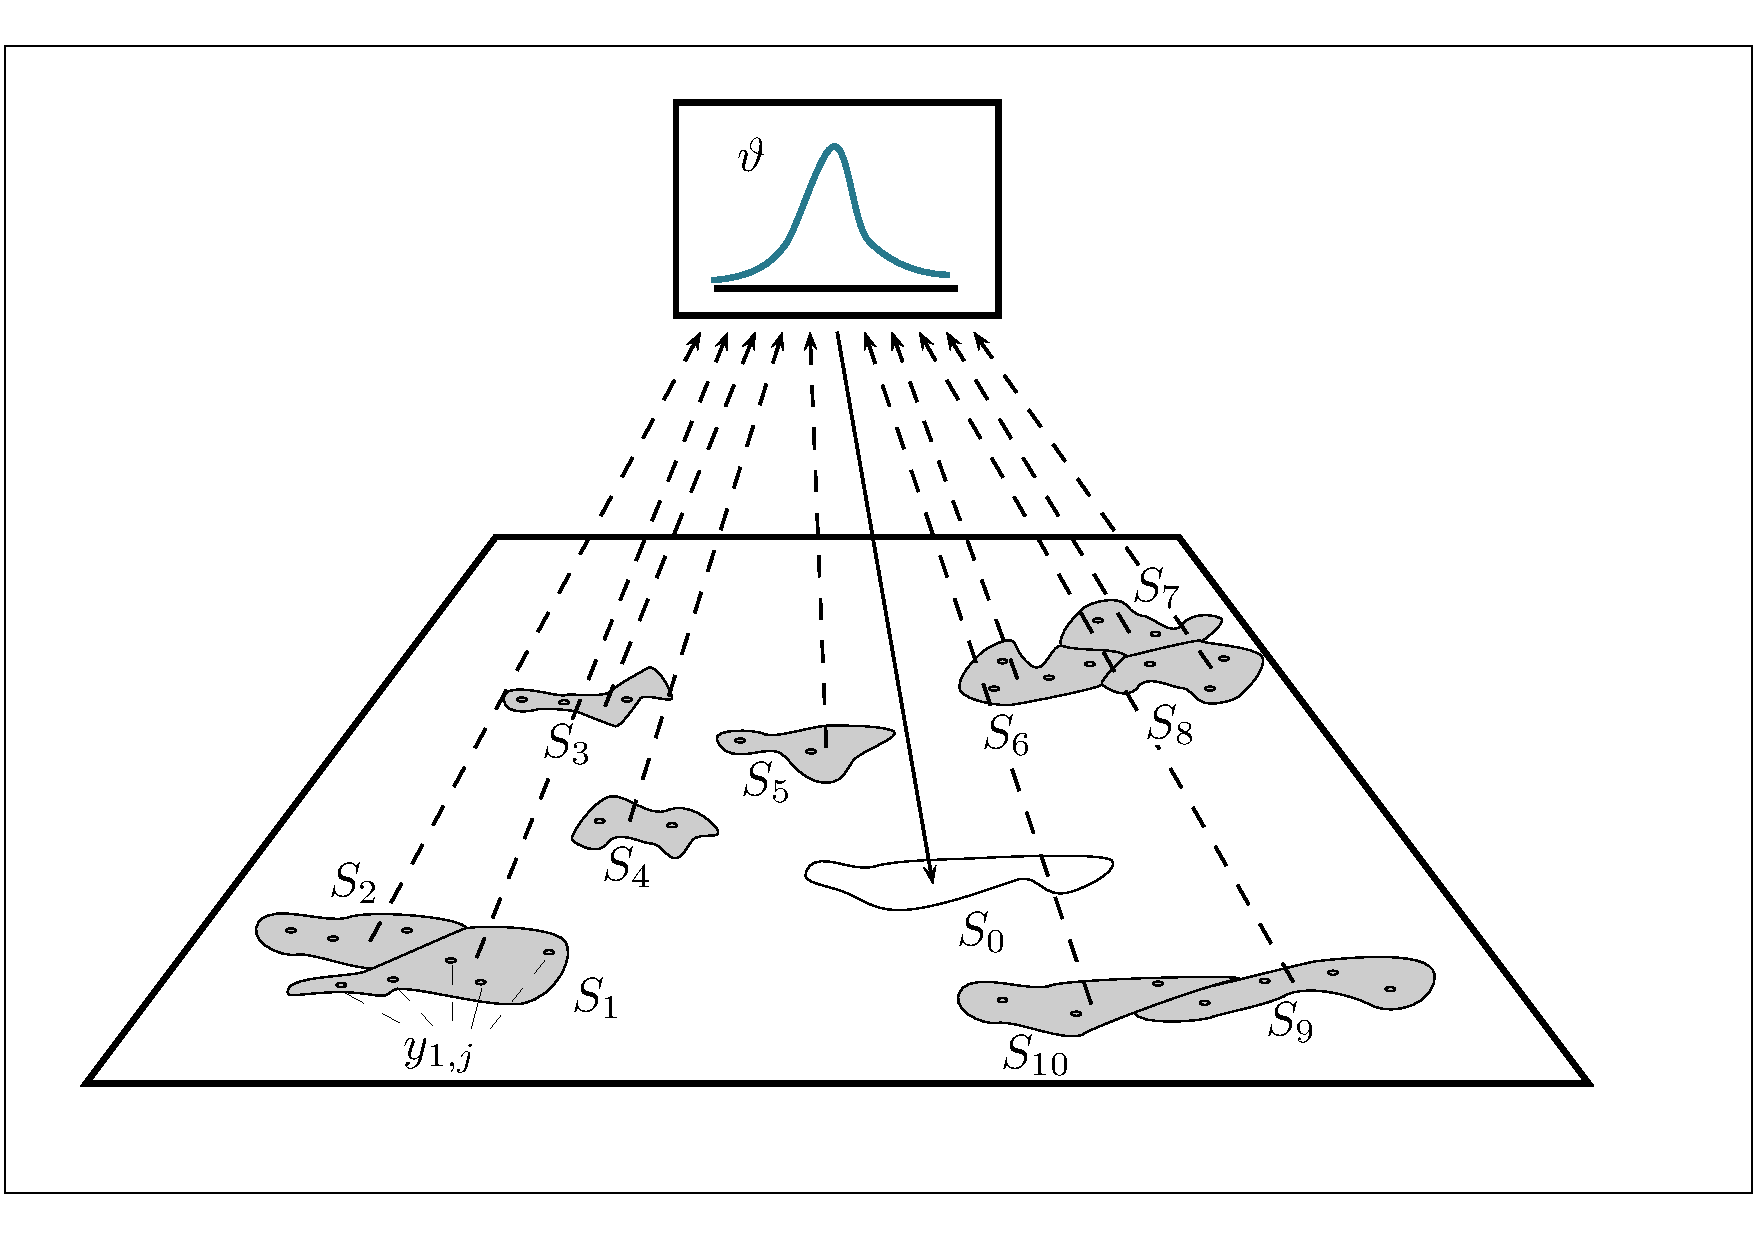
\includegraphics[width=1.0\textwidth]{img/regionalization.pdf}
    \caption{Schematic of the transfer of data from a number of donor sites $S_i$ to a new site $S_0$. Measurement locations are denoted by circles. The statistical model used for the transfer is denoted by its parameter vector $\vartheta$.}
    \label{fig:regionalzation}
\end{figure}

By definition, the prior distribution characterizes the knowledge about target parameters before observing in-situ data $y_{in}$. 
Therefore, $y_{in}$ cannot be used for the definition of the prior \citep{James2006}. 
On the other hand, using no data and making the prior distribution as vague as possible seems far too prudent since this would ignore the wealth of background knowledge which exists for virtually any geostatistical variable. 
Such background knowledge can come from data collected at other sites $S_i, i \in 1 \dots I$ (see schematic in Figure \ref{fig:regionalzation}). 
To distinguish them from the site-specific, in-situ data $y_{in}$, we use the term ex-situ data $y_{ex}$. 
Our prior pdf for the parameters at a new site $S_0$ could therefore be based on these ex-situ data $p(\theta|y_{ex})$. 
To determine this $p(\theta|y_{ex})$, we propose the use of a dedicated statistical model (more on this below). 
By virtue of this model, the transfer of information from known donor sites $S_i$ to a new site $S_0$ is a case of Bayesian prediction 
\begin{equation}
    \label{eq:pred}
    p(\theta|y_{ex}) = \int_{\vartheta} p(\theta|\vartheta) p(\vartheta|y_{ex}) d\vartheta.
\end{equation}

According to Eq. \ref{eq:pred}, the prior distribution  $p(\theta|y_{ex})$ for a new site $S_0$  is the posterior predictive distribution of all $S_i$ w.r.t. $S_0$ (see schematic in Figure \ref{fig:regionalzation}). 
Mathematically, this means $p(\theta|y_{ex})$ is derived by weighing each single predictive distribution $p(\theta|\vartheta)$ with its corresponding posterior distribution $p(\vartheta|y_{ex}) $ and marginalizing over the parameters $\vartheta$.
Please note the difference between the model for $X$ at site $S_0$, say a GP defined by $\theta$, and the model used for the transfer of data between sites defined by ${\vartheta}$. 
Since geostatistical data are hierarchical in nature, this model should be hierarchical too \citep{Kruschke2010, Gelfand2012, Gelman2013}. 


\subsection{Formulation of the hierarchical model}\label{ssec:formulation}

In geostatistics, a common way to conceptualize a hierarchical ordering of the data is by using two levels (see schematic in Figure \ref{fig:regionalzation}). 
The first level represents the population of the (spatially distributed) local data $y_{i,j}$ available on every given site $S_i$ whereas the second level represents the global population of all available sites. 
In such a two-level hierarchical model, this relationship is represented such that the set of parameters $\vartheta$ is split up into two subsets $\vartheta = (\phi, \eta)$ for level 1 and 2 respectively. 
The hierarchical relationship between these two levels is represented by factorizing their joint probability through the definition of conditional probability $p(\phi, \eta) = p(\phi|\eta) p(\eta)$. 
The general formulation of the two-level model would then look like the following:

\begin{subequations}
\label{eq:hier_ref}
    \begin{equation}
    \label{eq:hier_ref_Y}
        y_{i,j} \sim p(y|{\phi_i}),
    \end{equation}
    \begin{equation}
    \label{eq:hier_ref_phi}
        {\phi_i} \sim p({\phi}|{\eta}),
    \end{equation}
    \begin{equation}
    \label{eq:hier_ref_prior}
        {\eta} \sim p({\eta}).
    \end{equation}
\end{subequations}

This means that each datum $y_{i,j}$ is drawn from a distribution with parameters $\phi_i$, which are specific to site $S_i$ only. 
This distribution, therefore, represents the local variability of the data found within a given site or intra-site variability (Eq. \ref{eq:hier_ref_Y}). 
These local parameters ${\phi_i}$ are, in turn, drawn from a distribution specified by the global parameters called \emph{hyperparameters} ${\eta}$. 
These hyperparameters, therefore, represent the global variability between sites or inter-site variability (Eq. \ref{eq:hier_ref_phi}).

This general formulation allows to flexibly choose parametric models used for all distributions. 
Since $p(y|{\phi_i})$ represents the data, this distribution should fit the empirically observed frequencies of $y$. 
Depending on the geostatistical parameter of interest, a user can use, e.g., the normal, log-normal, multivariate normal, or truncated normal distributions to model parameter behavior. 
Choosing the distributions of the hierarchical model itself, i.e., $p({\phi}|{\eta})$ and $p({\eta})$ is less straightforward and should reflect of mixture of the domain knowledge and statistical expertise. 
To exemplify this procedure, let us look at measurements of hydraulic conductivity.
These data are often modeled with a log-normal distribution \citep{Hoeksema1985}, while $p({\phi}|{\eta})$ can be modeled as a normal distribution \citep{Gelman2013}. 
The parametric form of $p({\eta})$ should be specified as vague priors initially, with the posteriors being determined by the data $y_{ex}$. Transforming our data into their log-normal form, as often done, the resulting hierarchical model would then be

\begin{subequations}
\label{eq:hier_ex}
    \begin{equation}
        y_{i,j} \sim \mathcal{N}(\mu_i, \sigma^2),
    \end{equation}
    \begin{equation}
        \mu_i \sim \mathcal{N}(\alpha,\tau),
    \end{equation}
    \begin{equation}
        (\sigma^2, \alpha, \tau) \sim p(\sigma^2)p(\alpha)p(\tau).
    \end{equation}
\end{subequations}

In this example, we assumed that the variance $\sigma^2$ at each site is the same, making the local and global parameters identical. 
This assumption is, of course, a simplification but allows to reduce the number of parameters to be inferred.


\subsection{Generation of the ex-situ prior distribution}\label{ssec:general-structure}

Once the target variable is specified, and the ex-situ data $y_{ex}$ collected, three steps are necessary to actually calculate the prior distribution. 
First, the user has to decide on the parametric model for the distributions and therefore fully specify the hierarchical model according to Eq. \ref{eq:hier_ref}. 
Next, the posterior distributions of the parameters $p({\phi, \eta}|y_{ex})$ are inferred. 
In \CRANpkg{exPrior}, this is done using the Markov chain Monte Carlo (MCMC) implementation of \pkg{NIMBLE}.
Finally, the ex-situ prior can be determined as the posterior predictive distribution (see Equation \ref{eq:pred}). 

To familiarize ourselves with this procedure, let us look at these three steps in more detail.


\paragraph{Specifying a hierarchical model}\label{sssec:implementation}

The specification of the hierarchical model in \CRANpkg{exPrior} is done in \texttt{BUGS} code wrapped within the \pkg{NIMBLE} function \texttt{nimbleCode()}. 
The results are \texttt{R} objects from the \texttt{BUGS} models. 
In \pkg{NIMBLE}, every model is represented as a Directed Acyclic Graph (DAG), where each declaration in the model is a node which can be either deterministic or stochastic.
Nodes are represented as vertices of a DAG, with edges connecting nodes implying dependence relationships.

\begin{figure}[ht]
    \centering
    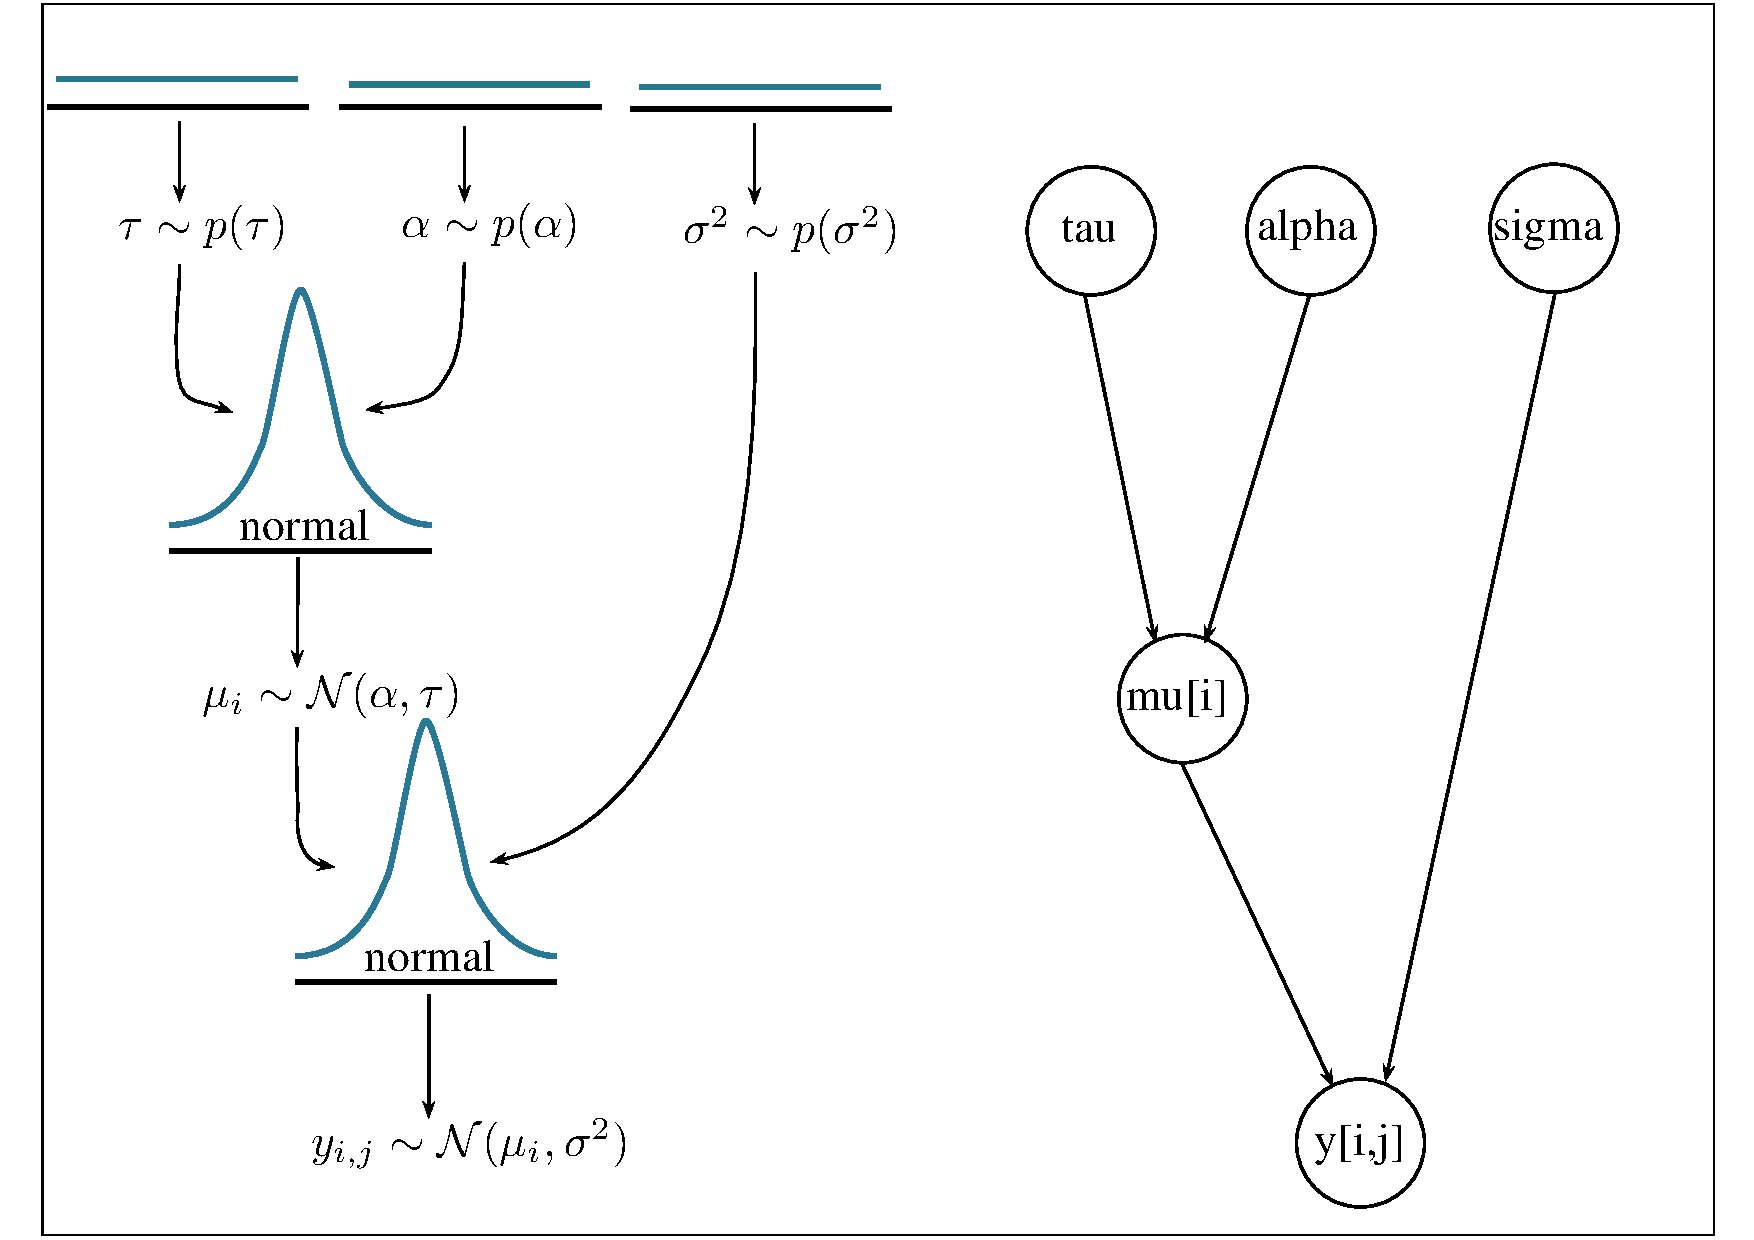
\includegraphics[width=1.0\textwidth]{img/hierarchical_example.pdf}
    \caption{Schematic of the example model showing the statistical model on the left as defined in see Eq. \ref{eq:hier_ex} and the corresponding DAG on the right. The arrows show the hierarchical relationships between the variables. Both the ex-situ data $y_{i,j}$, and the site-specific mean $\mu_i$ are drawn from normal distributions. The hyperparameters $\eta = (\tau, \alpha, \sigma^2)$ are given initially vague hyperpriors to be updated later by the ex-situ data.}
    \label{fig:model_workflow}
\end{figure}

To exemplify this, let us consider the aforementioned model for the log-hydraulic conductivity. 
As mentioned, the data at each site are modeled as being drawn from a normal distribution with every site having the same variance $\sigma^2$ but site-specific means. 
This mean value is again drawn from a normal distribution. 
Accordingly, $\alpha$ is the global mean of the local means, and $\tau^2$ represents the global variability of the local means. 
Since no data are used at this point, the hyperpriors of the hyperparameters $\eta = (\alpha, \tau, \sigma)$ should be non-informative.

The model is therefore declared with five variables: \texttt{alpha}, \texttt{tau}, \texttt{sigma}, \texttt{mu}, and \texttt{y}. 
Once compiled, the model contains multiple nodes: one node for each hyperparameter \texttt{alpha}, \texttt{tau}, and \texttt{sigma}, \texttt{I} nodes for the site-specific means \texttt{mu[i]}, and \texttt{$\sum_i{J_i}$} nodes for the site measurements \texttt{y[i,j]}. 
In this model, the dependent nodes are the ex-situ data $y_{i,j}$, the $\mu_i$ values are estimated from these deterministic $y_{i,j}$. 
Similarly, the $\alpha$ and $\tau$ are estimated from the $\mu_i$. 
In cases where the data are provided to \texttt{genExPrior()} in the form of moments (more on this later), \texttt{mu[i]} is deterministic, as the site-specific means are already provided in numeric form and not considered to be realizations from any distribution. 
The following pseudocode illustrates how the model is declared:

\begin{example}
## declaration of a hierarchical model in nimbleCode

# 1. declare prior distributions for hyperparameters
hyperparameters ~ disn(...)

# 2. declare distributions for site-specific means
for i in 1:I {
  mu[i] ~ disn(hyperparam1, hyperparam2, ...) # distribution of mean mu at site i
  
# 3. declare distributions for measurements
  for j in 1:J {
  y[i,j] ~ disn(mu[i], hyperparam3, ...)
  }
}
\end{example}

%\verbatiminput{output/generalFromMeas_code.txt}

This pseudocode model denotes the mathematical formulation of the hierarchical model in BUGS code, where the parameter for site-specific means $\mu_i$ is \texttt{mu[i]}, and site-specific variances $\sigma^2_{i}$ is \texttt{sigma2[i]}. 
First, hyperparameters \texttt{alpha} and \texttt{tau} are assigned non-informative hyperpriors. 
Next, the code loops through each site and assigns the mean \texttt{mu[i]} a distribution whose parameters are hyperparameters. 
Finally, each of the \texttt{J} measurements \texttt{y[i,j]} at each site \texttt{i} is assigned a distribution with parameters \texttt{mu[i]} and hyperparameters. 

The flexibility of this formulation allows the data $y_{ex}$ to be assimilated in a full MCMC hierarchical model, as explained in the next section.


\paragraph{Estimating posterior values of parameters in the hierarchical model}

Parameters in the hierarchical model are estimated from the data provided by the user, using MCMC. 
Once the model and the variables are declared, the hierarchical model is compiled using \texttt{nimble::compileNimble()}. 
The MCMC object is configured, built, and compiled using \texttt{nimble::configureMCMC()}, \texttt{nimble::buildMCMC()}, and \texttt{nimble::compileNimble()}, respectively and run using the run method of the compiled object. 
This method calculates an MCMC chain, the result of the estimation step. 
To improve numerical efficiency, NIMBLE includes a library of algorithms and a compiler that generates C++ for declared models and functions. 
Once a model is declared, \texttt{nimbleCode} is generated as C++ code, compiled, and reloaded into R.

The values in the compiled model are declared with data that are supplied by the user when running the function. 
For example, if a user inputs a data frame of measurements, each of the \texttt{y[i,j]} is defined with its corresponding data point. 
If a user provides moments, then each of the \texttt{mu[i]} is defined with its provided value. 
Once a model is compiled, \texttt{genExPrior()} envokes the MCMC sampler, which estimates the posterior distributions of the parameters. 

\paragraph{Predicting the prior}

Now that the ex-situ data are assimilated, our hierarchical model is fully conditioned on all available data. 
Normally, this would conclude a Bayesian inference. 
Yet as explained above, the posterior distribution has to be used to compute the predictive posterior distribution of the target variable at a new site (see Eq \ref{eq:pred}). 
In \CRANpkg{exPrior}, this is simply done by drawing realizations of the target variable from distributions specified by the hierarchical model and parameterized by values sampled from the MCMC chains from the previous step. 
The final predictive posterior distribution is then estimated using kernel density estimation. 


% ======================================================================================= %
% Section 3
% ======================================================================================= %

\section{Associated packages}

To support the functionality of \CRANpkg{exPrior}, we provide two additional R packages on the GitHub account.
First, the \pkg{geostatDB} package provides real-world data on subsurface measurements, which can therefore be used directly for the derivation of informed prior distributions.
Second, the \pkg{siteSimilarity} package allows users to determine a cluster of similar sites to focus on the most relevant data only and therefore reducing the overall uncertainty.
Since both these packages provide benefits independently of \CRANpkg{exPrior}, they will remain independent for the foreseeable future.


\subsection{Real-world data: The \pkg{geostatDB} package}

In this package, we provide real-world, geostatistical data from the WorldWide HYdrogeological Parameters DAtabase \textit{WWHYPDA} \citep{Comunian2009}.
This database has been designed to store values of the most important properties of earth materials and has been developed with the purpose of offering a complement of information in hydrogeological studies where there is a lack of data. 
To the best of the authors' knowledge, the WWHYPDA is the largest open-source database of hydrogeological parameters. 
Currently it contains a total of 20,523 subsurface measurements of 6 geostatistical parameters spanning 128 sites. 
A complete description and schematic of the database in its original form can be found in \citet{Comunian2009}.

Due to its size, as well as to facilitate further additions to the database, we use a dedicated R package \pkg{geostatDB} to host the data from WWHYPDA.
This package is not yet on CRAN, but the latest release version can be found on \url{https://github.com/GeoStat-Bayesian/geostatDB} \citep{geostatDB_zenodo}.
To exemplify the usage and impact of real-world data, we furnished \CRANpkg{exPrior} with an example data set on porosity values from sandy aquifers. 
Its usage is described in Section \ref{ssec:using-exPrior} below.

\pkg{geostatDB} itself includes the WWHYPDA as an SQLite database, converted from the online MySQL database. 
The reasons for using SQLite are efficiency and accessibility. 
First, both SQL and SQLite databases can be easily read into \texttt{R}, while maintaining their original structure. 
SQLite specifically can be included in R packages without the need for a server, making it accessible to the user. 
A downside of this decision is that a user who updates the SQLite database in \pkg{geostatDB} does so without making changes to the original database, hosted on \url{https://www.wwwhypda.org}.
Thus, those who wish to contribute to the WWHYPDA are currently encouraged to do so by submitting data online.

\begin{figure}
    \centering
    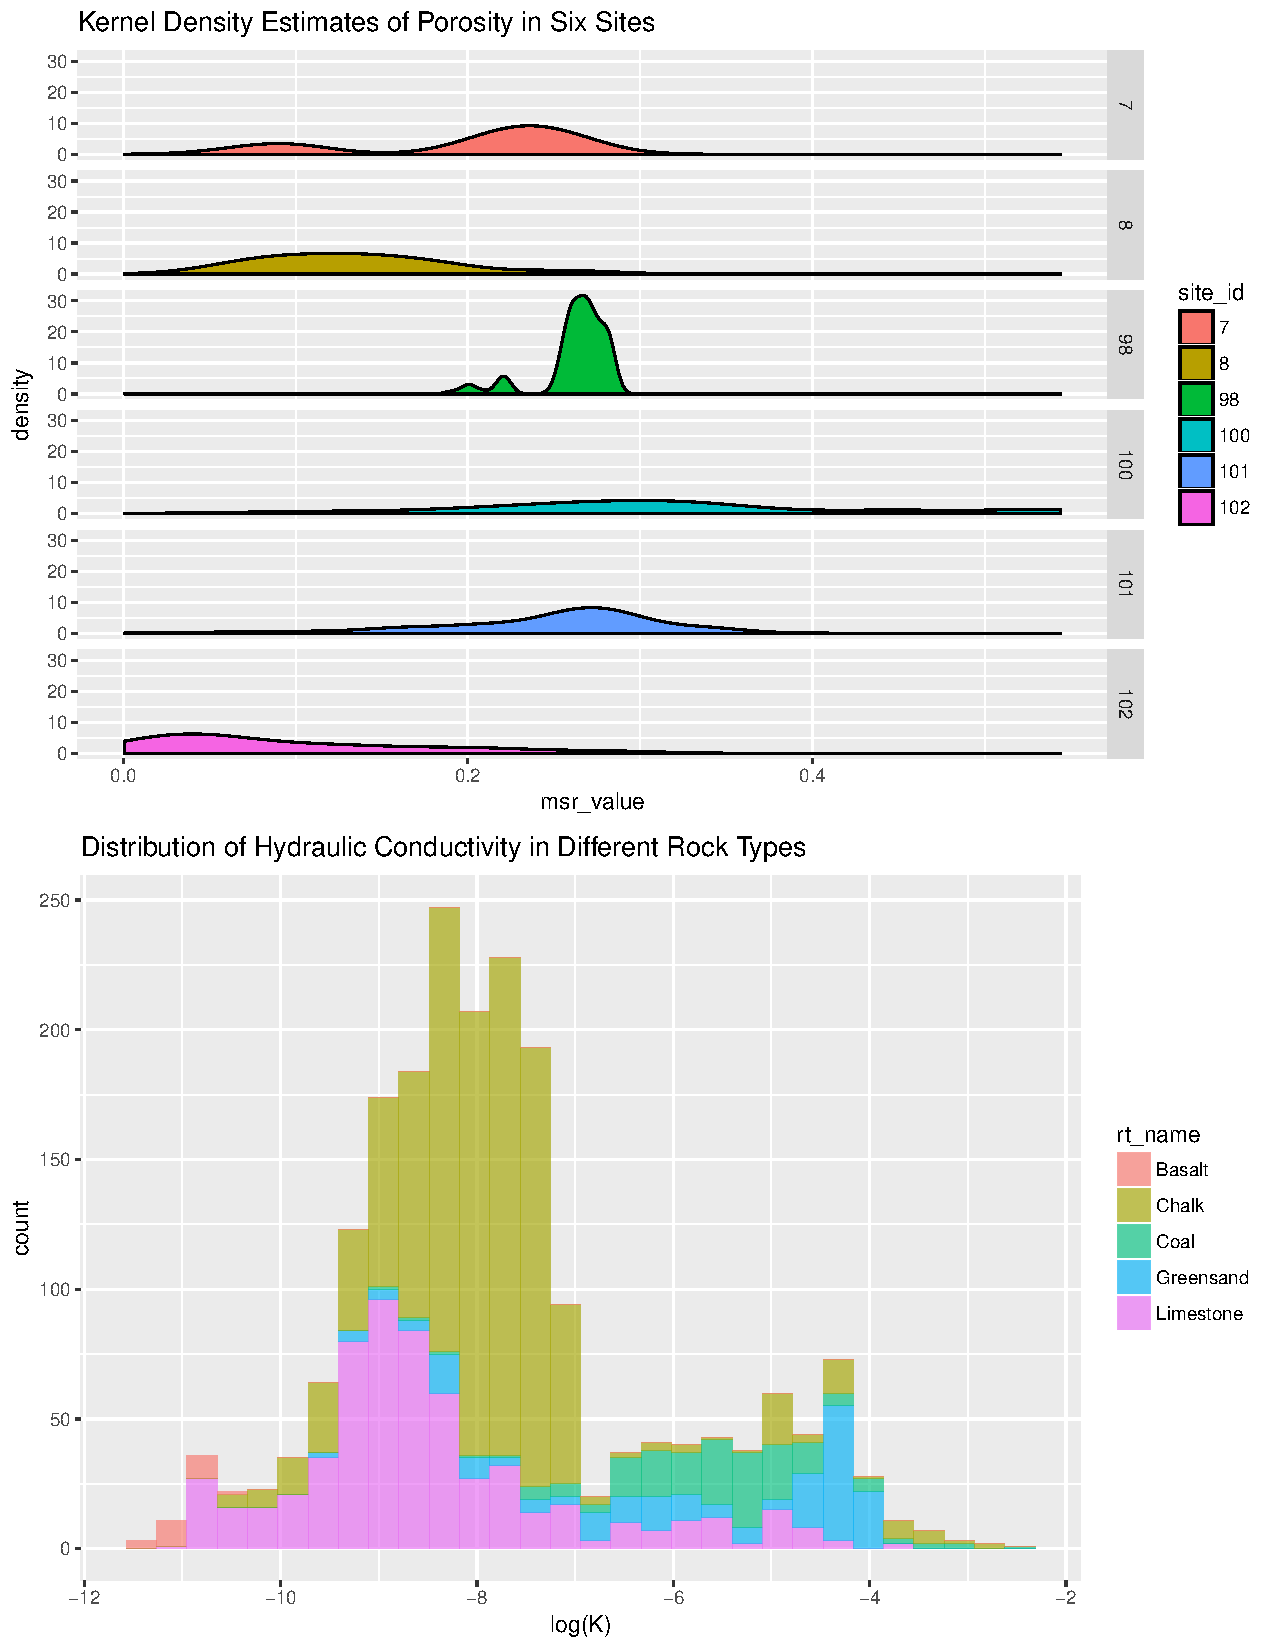
\includegraphics[width=\textwidth]{img/wwhypda_vis_2.pdf}
    \caption{The two visualizations are made using the data from the WWHYPDA, obtained using the function \texttt{getData()} from the \pkg{geostatDB} package. The first figure shows the distribution of porosity values at several sites, derived using kernel density estimation. The second figure shows a set of histograms describing the distribution of hydraulic conductivity values for different material types.}
    \label{fig:wwhypda}
\end{figure}

It is important to note that data quality steps need to be implemented before applying the statistical algorithm to this database. 
%Some fields have missing values, and some names of sites are not clean. 
Figure \ref{fig:wwhypda} contains two visualizations that describe the data present in the WWHYPDA, created in \texttt{R}.
This visualization was done using the function \texttt{getData()} from the \pkg{geostatDB} package.
The code can be found in the associated vignette of the package at \url{https://github.com/GeoStat-Bayesian/geostatDB/blob/master/vignettes/explore_data.Rmd}.


\subsection{The notion of site similarity: The \pkg{siteSimilarity} package}

In order to reduce the uncertainty in the prior distribution as much as possible, it is beneficial to focus only on data coming from sites which are similar to the one under investigation.
It is therefore crucial to have a sound notion of site similarity.
The \pkg{siteSimilarity} package uses hierarchical agglomerative clustering to categorize sites into clusters based on observable characteristics, such as environment type or rock type. 
Using the schematic in Figure \ref{fig:regionalzation}, only those sites similar to site $S_0$ would be used as donor sites.
Currently, the clustering achieves only a modest reduction in uncertainty when using a leave-one-out validation.
This is caused by the overall limited number of sites, which, after clustering, get even more reduced.
Yet the algorithm already provides the user with a tangible benefit, which is projected to increase as more and larger data sets with more sites become available. 

% =================================================================================== %
% Section 4: Examples
% =================================================================================== %

\section{Examples}

Having now formally explained the workflow and associated packages of \CRANpkg{exPrior}, we will illustrate said workflow with a series of examples. 
Starting with an easy inference problem, we will then explain how to use the included data, how to account for autocorrelation, and finally how to use soft data, in particular bounds, for the inference. 

Please note that all examples given in the following only refer to the distribution of the expected quantity itself, e.g., porosity. 
This does, however, not mean that the parameters of a GP cannot be inferred since $\mu$ and $\sigma$ are nodes in the hierarchical model and can be derived from it. On the other hand, higher-order statistics, like correlation length or anisotropy, are usually considered homogeneous across a given site and are consequentially not hierarchical. 
They can, therefore, be inferred using the classical estimation procedure.

The following four examples correspond to four vignettes, which can be found on the GitHub account of the \pkg{exPrior} package at \url{https://github.com/GeoStat-Bayesian/exPrior/blob/master/vignettes}.

\begin{figure}[ht]
    \centering
    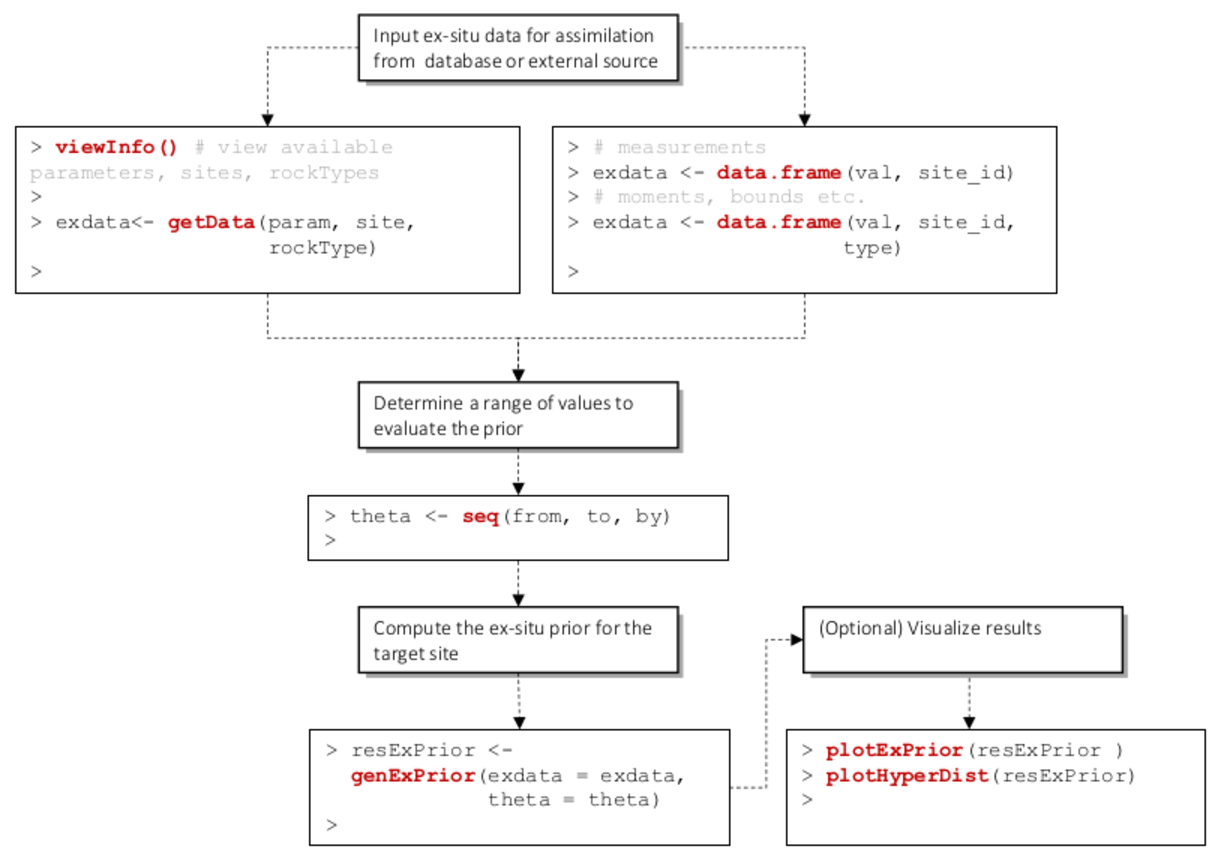
\includegraphics[width=1.0\textwidth]{img/package_workflow.pdf}
    \caption{A flowchart showing the workflow of the user of \CRANpkg{exPrior}. A user first expresses ex-situ data as an R dataframe. The user then determines the range of values at which to compute a prior (usually the minimum and maximum values of a parameter). Finally, the user uses \texttt{genExPrior()} to compute the ex-situ prior for a target site. The user has the options of using built-in plotting functions to visualize results.}
    \label{fig:package_workflow}
\end{figure}

The general workflow, which is followed in all of these examples, is visualized in Figure \ref{fig:package_workflow}. 
First, a user has to represent the ex-situ data in the form of an \texttt{R dataframe} object.
These data can be manually entered, like explained in Section \ref{ssec:quick-example}, taken from the included data, like explained in Section \ref{ssec:using-exPrior}, or being supplied though some additional database. 
Next, the user would enter as an \texttt{R vector} object a range of values at which to estimate the prior distribution. 
This range is typically the minimum and maximum values of the parameter of interest (for example, porosity takes values between 0 and 1). 
Finally, the user would input the ex-situ data and specified range into the function \texttt{genExPrior()}, which outputs a prior and the distributions of hyperparameters of the model.
The user has the options of using built-in plotting functions to visualize results.


\subsection{Example 1: Using \CRANpkg{exPrior} with synthetic data}\label{ssec:quick-example}

To familiarize the reader with this general workflow, let us start with a simple example using only a few synthetic data (on a log 10 scale) from three arbitrarily labeled sites $S_1$, $S_2$, and $S_3$.
The source code for the corresponding vignette can be found at \url{https://github.com/GeoStat-Bayesian/exPrior/blob/master/vignettes/using_genExPrior.Rmd}. 
The goal is to derive the ex-situ prior for target site $S_0$ with the following code:

\begin{example}
> exdata <- data.frame(val = c(c(-2,-3,-4), c(-2,-1), c(-6,-7,-2,-3)), 
+                      site_id = c(rep('S1',3), rep('S2',2), rep('S3',4))) 
> ex_prior <- genExPrior(exdata = exdata, theta = seq(from=-10, to=10, by=0.1)) 
\end{example}

By following the above workflow, we started with generating an \texttt{R dataframe} \texttt{exdata} for the ex-situ data. 
Then, we entered the range over which to estimate the variable $\theta$ as an \texttt{R vector} \texttt{theta}. 
The actual computation of the ex-situ prior is finally performed by the function \texttt{genExPrior()}. 
To investigate the output of this function, \CRANpkg{exPrior} provides a number of plotting functions.

%Here, the output for each node \texttt{mu[1], mu[2]} and \texttt{mu[3]} comes from the function \texttt{configureMCMC()}, which detects the conjugacy of each node and samples from its posterior distribution. The computation speed depends on both the number of sites and the number of measurements a user wishes to assimilate. 


%To investigate the prior distribution the function \texttt{plot\_exPrior} is availbale whereas the posteriors of the hyperparameters can be visualized with the function \texttt{plotHyperDist}

\begin{example}
> plotHyperDist(ex_prior) 
> plotExPrior(ex_prior) 
\end{example}

\begin{figure}
    \centering
    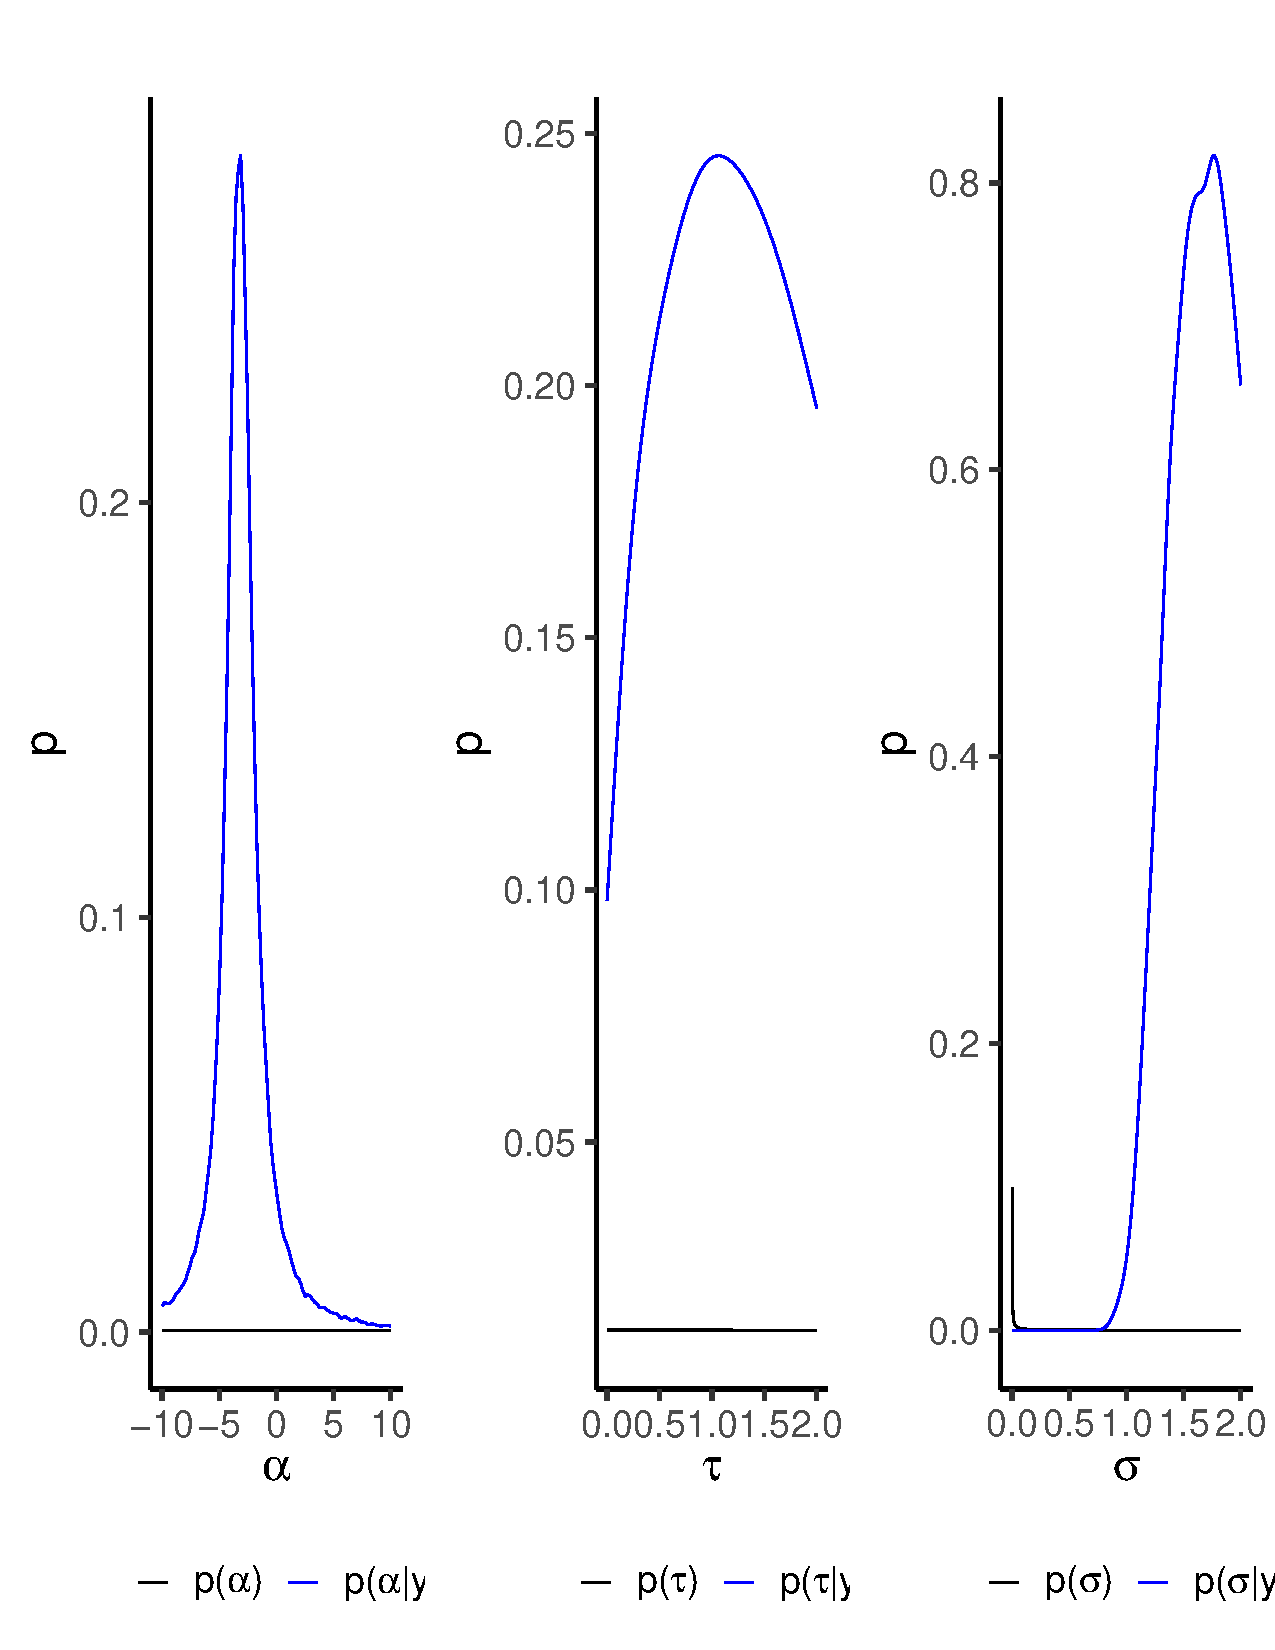
\includegraphics[width=0.45\textwidth]{img/example_1_hyperDist.pdf}
    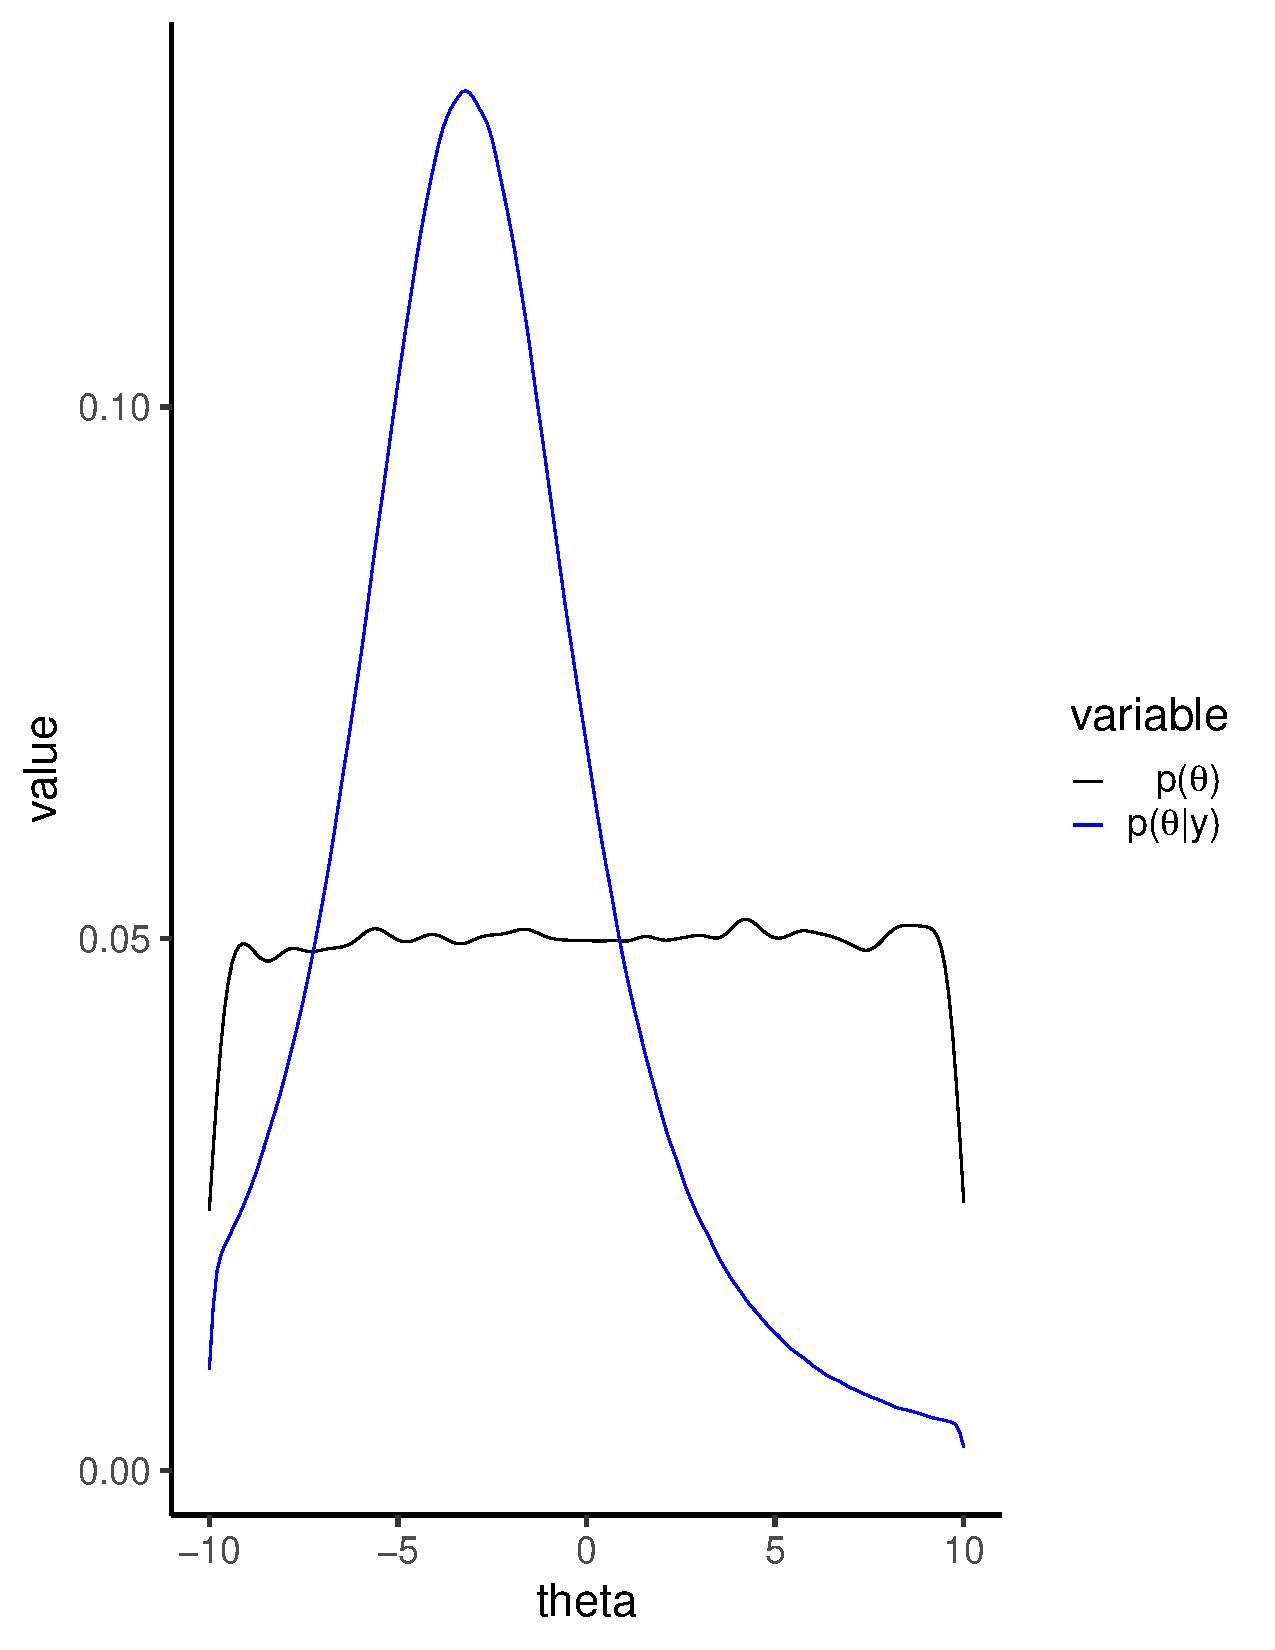
\includegraphics[width=0.45\textwidth]{img/example_1_exPrior.pdf}
    \caption{The left panel shows the distributions of the hyperparameters \texttt{alpha}, \texttt{tau}, and \texttt{sigma}. The right panel shows ex-situ prior computed using the data assimilation framework (blue curve) against the uninformative prior (black curve).}
    \label{fig:quick_example_prior}
\end{figure}

In this little example, the first command \texttt{plotHyperDist} plots the posterior distributions of the hyperparameters $\alpha$, $\tau$, and $\sigma$ (see Figure \ref{fig:quick_example_prior} left panel). 
This captures the impact of the data on the Bayesian hierarchical model. 
The second command \texttt{plotExPrior} shows the ex-situ data from the three sites jointly with the predicted prior distribution for the new site $S_0$ (see Figure \ref{fig:quick_example_prior} right panel). 
As can be seen, the essentially flat, uninformative prior got updated into a much sharper, informative prior representing a much-reduced uncertainty.

\subsection{Example 2: Using \CRANpkg{exPrior} with real-world data}\label{ssec:using-exPrior}

%As introduced above, \CRANpkg{exPrior} provides real-world geostatistical data from the wWWHYPDA as well as methods for accessing these data using R with the functions \texttt{viewInfo()} and \texttt{getData()}, removing the need for SQL knowledge. %[KARINA: worth noting that these functions suppose that the database was downloaded to the machine of the user, as there is currently no API for querying that data.... If the user doesn't want to do that, we also provide the data as an R dataframe in the package]. 
%The former function returns an R list that describes  the contents of the database, and the latter function queries the database to return user-specified information. 
%The functions both rely on the package \CRANpkg{RSQLite}, which connects \texttt{R} to a SQLite database. 
%Given that the database is included in the package, a user that is familiar with SQL has the option of connecting to the database directly using \pkg{RSQLite}.% [KARINA: To be confirmed with Nura, but I don't think this is true (I had a look in the package). We provide the data as an R dataframe, but not as an SQL database.]. 

%\texttt{viewInfo()} allows the user to view information about the database, including a list of tables (excluding those that are empty), a list of entered parameters, sites and rock types as well as a relational schema.

%While this function shows information about the database, it does not allow a user to query it.
%The function \texttt{getData()} sends a query to the \textit{WWHYPDA} that joins multiple tables to return one large \texttt{R dataframe} containing 39 columns and 20523 rows.

%A user can specify parameters, rock types and sites of interest by adding arguments to \texttt{getData()}. 

As introduced above, \CRANpkg{exPrior} provides real-world, geostatistical data from the WWHYPDA.
Let us exemplify its use and impact on the inference by first importing the data on porosity.
As above, the associated vignette can be found at \url{https://github.com/GeoStat-Bayesian/exPrior/blob/master/vignettes/real_world_data.Rmd}.

\begin{example}
> load(file="data/df_porosity.rda")
\end{example}

These real-world data are now loaded into the workspace and can be used to compute the ex-situ prior using the `exPrior` function as describe in above example

\begin{example}
> resExPrior = genExPrior(exdata = df_porosity, theta = seq(from=0, to=1, by=0.01))
\end{example}

Here, the range of the \texttt{theta} vector reflects the common-sense intuition that porosity values can only exist between 0 and 1. 
This change should also be reflected in the used model

\begin{subequations}
\label{eq:wwhypda}
    \begin{equation}
    \label{eq:wwhypda_a}
        y_{i,j} \sim \Phi(\mu_i, \sigma^2, 0, 1),
    \end{equation}
    \begin{equation}
        \mu_i \sim \mathcal{N}(\alpha,\tau),
    \end{equation}
    \begin{equation}
        (\sigma^2, \alpha, \tau) \sim p(\sigma^2)p(\alpha)p(\tau).
    \end{equation}
\end{subequations}

Equation (\ref{eq:wwhypda_a}) makes this change clear, such that the data are drawn from a truncated normal distribution. 
Since the boundaries are fixed, the hierarchical model itself still has the same number of parameters, and the other parts of the model remain the same.

After the completion of \texttt{exPrior}, we can visualize again the posteriors of the model as well as the prior of $\theta$ using \texttt{plotExPrior}. 

\begin{example}
> plotHyperDist(resExPrior)
> plotExPrior(resExPrior)
\end{example}

\begin{figure}
    \centering
    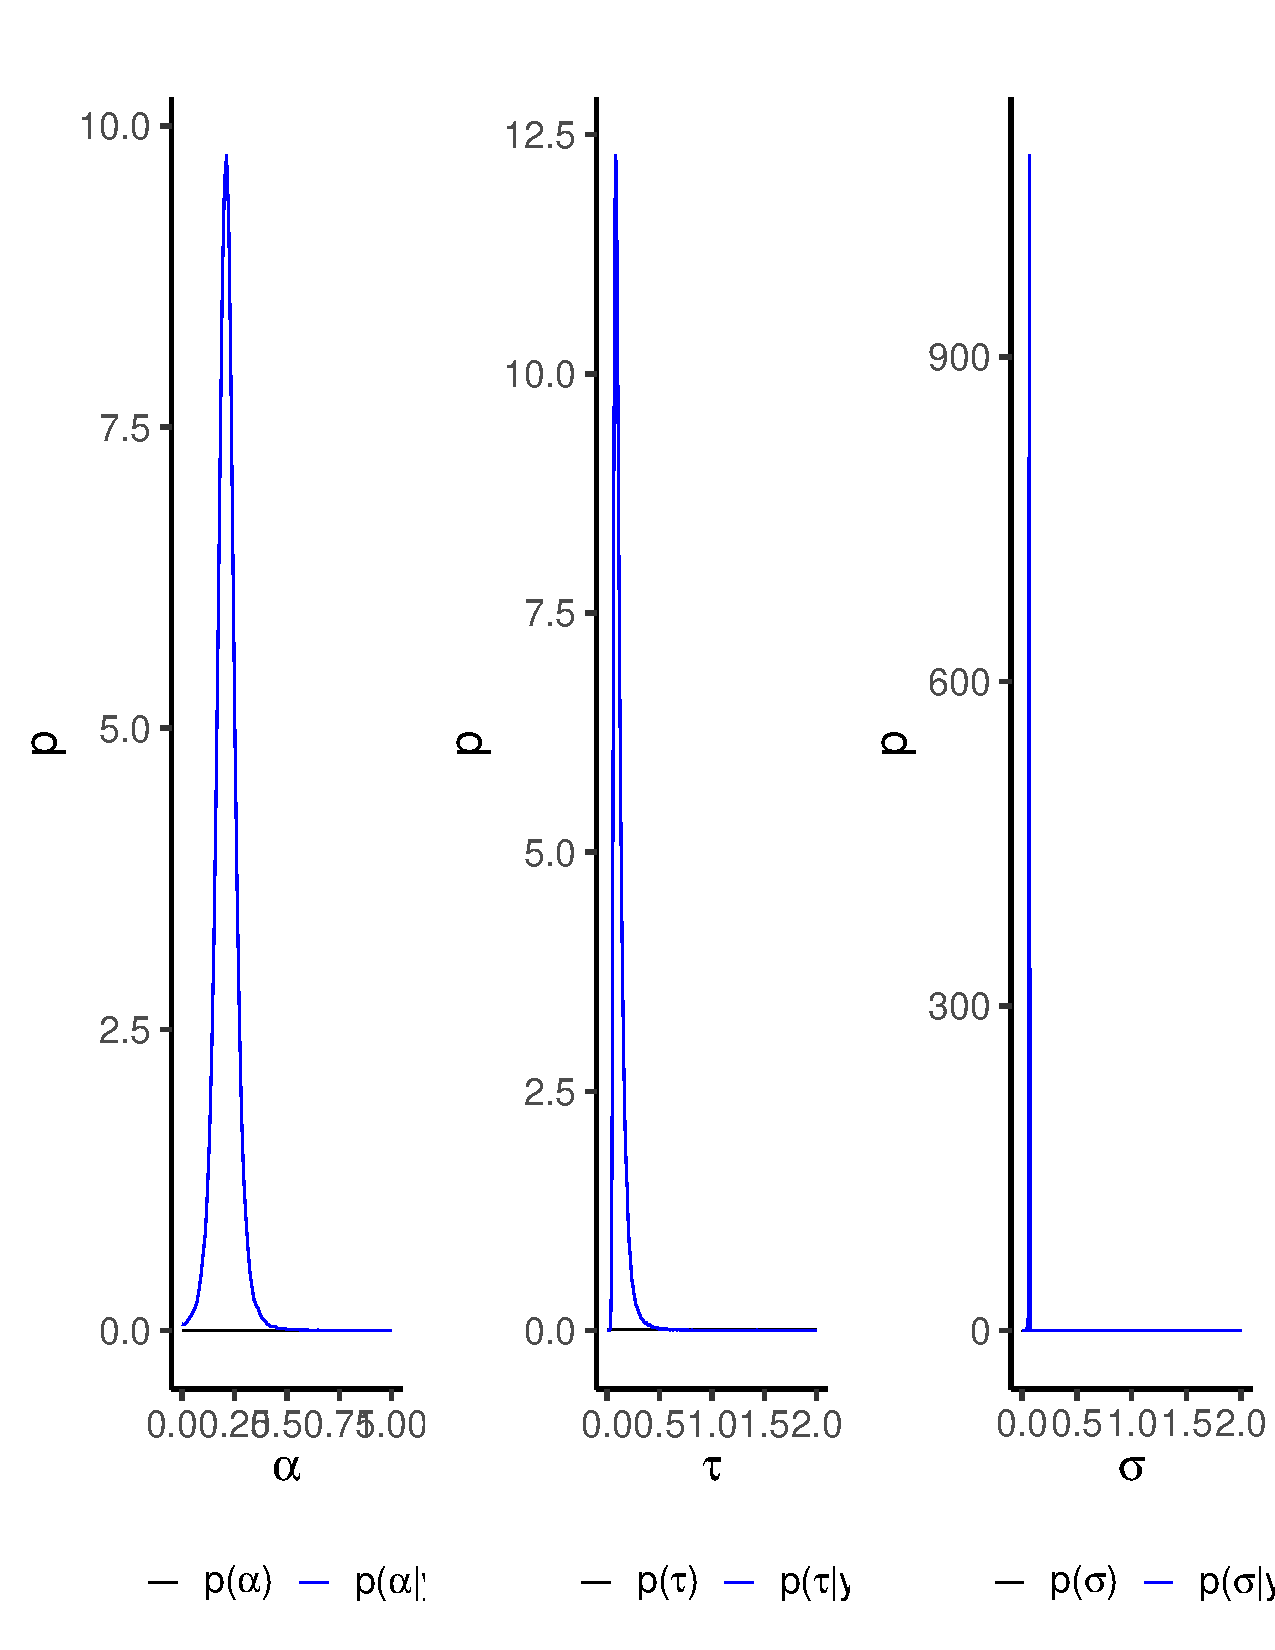
\includegraphics[width=0.45\textwidth]{img/example_2_hyperDist.pdf}
    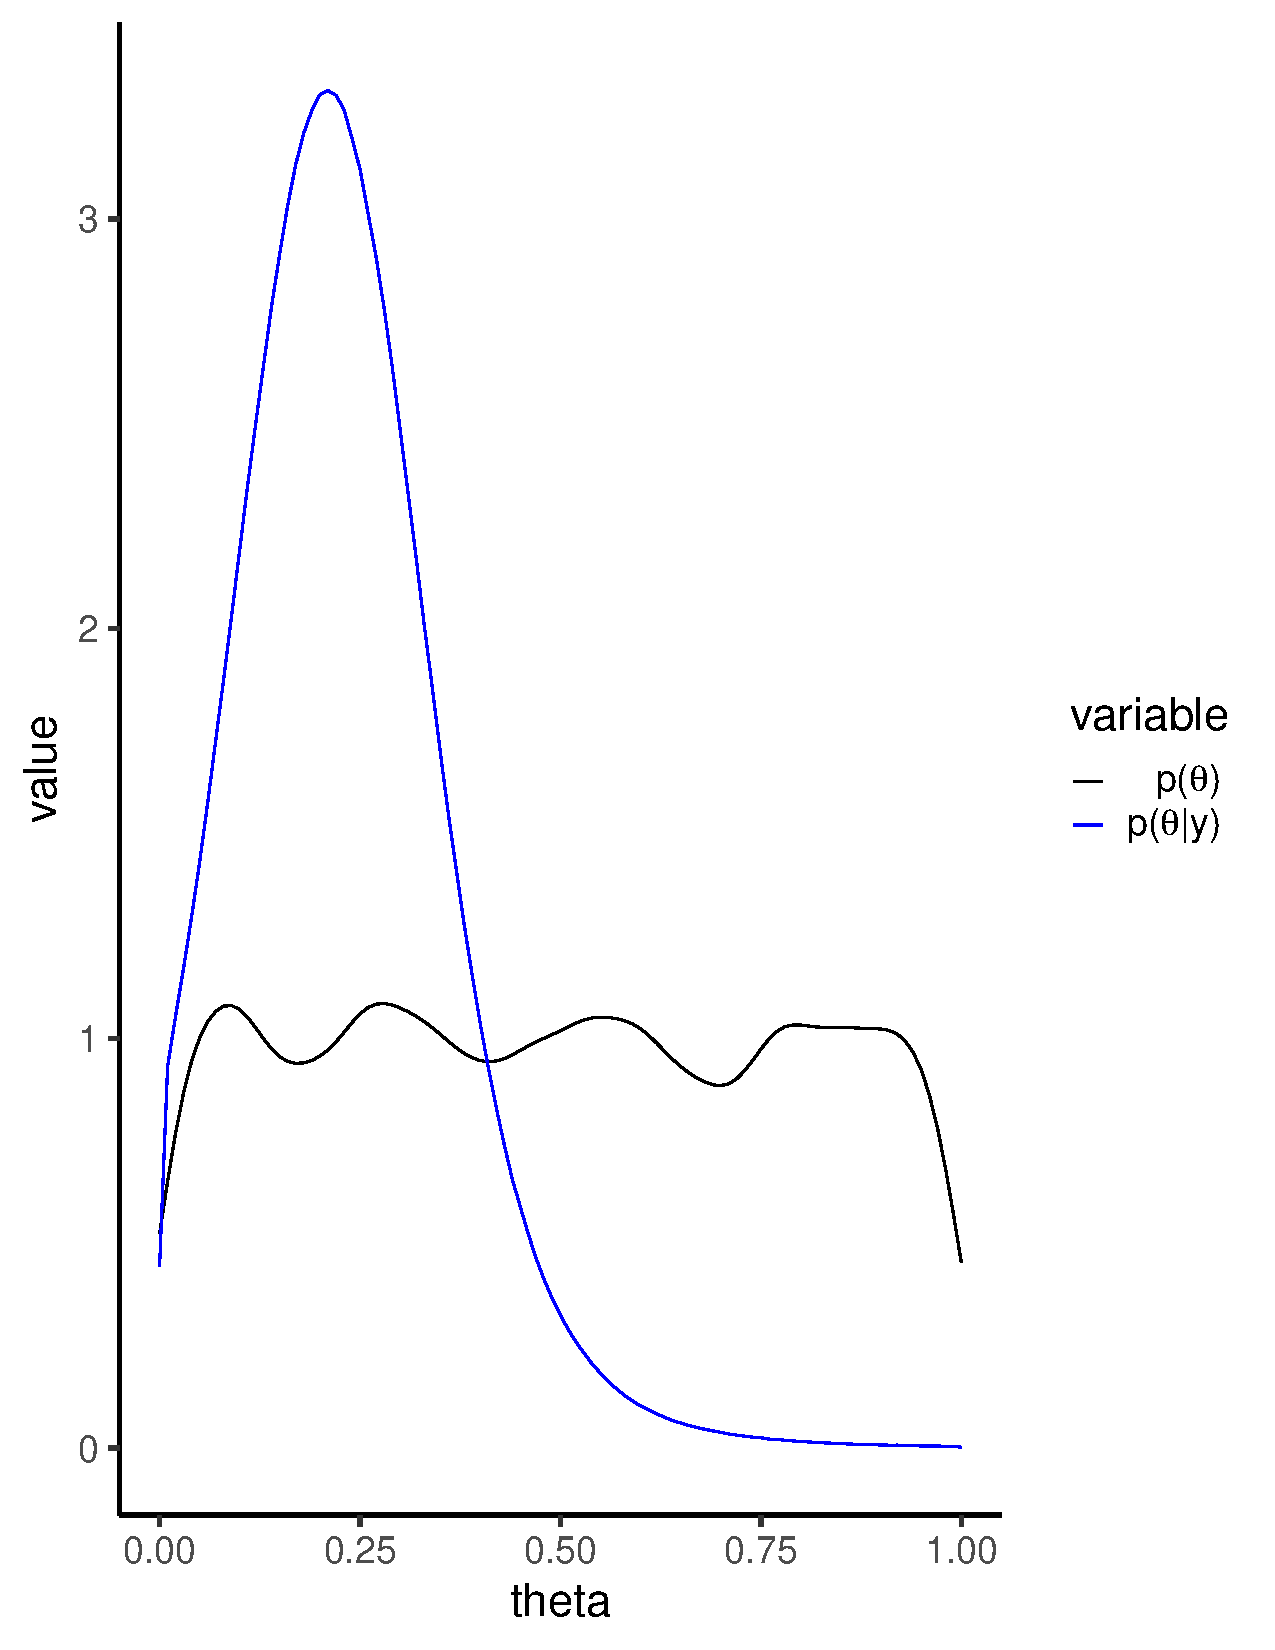
\includegraphics[width=0.45\textwidth]{img/example_2_exPrior.pdf}
    \caption{Informative (blue) and non-informative (black) priors computed with \texttt{genExPrior()} using real-world, ex-situ data of porosity in sand stone.}
    \label{fig:wwhypda_exprior}
\end{figure}

Compared to Figure \ref{fig:quick_example_prior}, the results in Figure \ref{fig:wwhypda_exprior} show some relevant differences. 
In particular, the hyperpriors seen in the left panel of Figure \ref{fig:wwhypda_exprior} are much more peaked, resulting in near-certainty about their value. 
This is due to the large amount of evidence provided by the data. 
Since the parameter distributions on the higher levels in a hierarchical model represent the uncertainty about the parameters on the lower ones, it can be said that the results of this inference capture the uncertainty of porosity in sandstone with high certainty. 
This means that the prior distribution in the right panel of Figure \ref{fig:wwhypda_exprior} is very close to the statistical uncertainty for the hypothetical population of all porosity values in sandstone aquifers in general. 
As can be seen in this figure, this distribution is strongly peaked between 0.2 and 0.3. 
Using this prior therefore provides a practitioner with a sound foundation for the geostatistical inference of the in-situ porosity. 


\subsection{Example 3: Accounting for spatial autocorrelation in ex-situ data} \label{sec:example-spatial}

In most cases, ex-situ data used in the analysis are spatially correlated since measurements are usually collected in a clustered way \citep{Rubin2003, Pyrcz2002}. 
The data assimilation model outlined in \ref{ssec:formulation} can, in principle, account for patterns of spatial variability by using multivariate distributions as site-specific distributions. 
As above, the associated vignette can be found at \url{https://github.com/GeoStat-Bayesian/exPrior/blob/master/vignettes/spatial_correlation.Rmd}.
To account for this spatial correlation, let us use a revised version of the hierarchical model from Equation (\ref{eq:hier_ex})

\begin{subequations}
\label{eq:hier_geospatial}
    \begin{equation}
    \label{eq:y_ij_MVN}
        y_{i,j} \sim \mathcal{N}(\mu_i,\Sigma),
    \end{equation}
    \begin{equation}
    \label{eq:mu_i_N}
        \mu_i \sim \mathcal{N}(\alpha,\tau),
    \end{equation}
    \begin{equation}
    \label{eq:Sigma}
        \Sigma = \sigma^2 \exp\bigg( -\frac{h}{\lambda}\bigg),
    \end{equation}
    \begin{equation}
    \label{eq:variogram_function}
         (\sigma^2, \lambda, \alpha, \tau) \sim p(\sigma^2)p(\lambda)p(\alpha)p(\tau).
    \end{equation}
\end{subequations}

The relevant adjustment can be seen in Equation (\ref{eq:y_ij_MVN}), where the data are no longer modeled to be drawn from a univariate normal distribution but a multivariate distribution instead. 
The main difference is the replacement of the variance $\sigma^2$ by the covariance $\Sigma$. 
In our example, this covariance is modeled as an isotropic exponentially decaying function, with a characteristic length scale $\lambda$. 
This function means that measurements being taken at large distances $h$ are essentially independent, and no relevant difference to the simple univariate model from Equation (\ref{eq:hier_ex}) would exist. 
However, measurements taken at distances $h$ similar or smaller to $\lambda$ exhibit substantial correlation and must be assimilated accordingly. 
Failing to do so would result in an underestimation of the actual uncertainty, a phenomenon which is known in the literature as pseudoreplication \citep{Hurlbert1984, Legendre1993}. 
Due to the additional parameter, the model has now 4 hyperparameters, which need to be inferred.

To exemplify the workflow with this revised hierarchical model, let us use synthetic data coming again from three different sites only. 
To generate data with spatial correlation, we used the \CRANpkg{gstat} package.
These synthetic data were then transformed to have different mean values for each site.

\begin{example}
> set.seed(1)
> xy <- data.frame("x" = sample(seq(0.00,1.00,0.01),22),
+                  "y" = sample(seq(0.00,1.00,0.01),22))
> model = vgm(psill=1, range=1, model='Exp')
> g.dummy <- gstat(formula=z~1, locations=~x+y, dummy=TRUE, beta=1, model=model, nmax=20)
> exdata_spatial <- predict(g.dummy, newdata=xy, nsim=1)
\end{example}

To adapt this data frame from \CRANpkg{gstat} to the format needed for \CRANpkg{exPrior}, we have to change one of the column names and add the site's id.

\begin{example}
> colnames(exdata_spatial)[3] <- "val"
> exdata_spatial\$site_id = c(rep("S1", 10), rep("S2", 5), rep("S3", 7))
> exdata_spatial[ 1:10, 'val'] <- exdata_spatial[ 1:10, 'val'] - 3
> exdata_spatial[11:15, 'val'] <- exdata_spatial[11:15, 'val'] - 2.5
> exdata_spatial[16:22, 'val'] <- exdata_spatial[16:22, 'val'] - 3.5
\end{example}

With these data, we can now generate the ex-situ prior distribution. 
To tell \CRANpkg{exPrior} to account for the spatial correlation in the data, we have to toggle the \texttt{spatialCoordinates} flag in the \texttt{genExPrior()} function to \texttt{TRUE}.

\begin{example}
> resExPrior = genExPrior(exdata = exdata, theta = seq(from=-10, to=10, by=0.1), 
+                         spatialCoordinates = TRUE)
> plotExPrior(resExPrior, plotExData = TRUE)
\end{example}

\begin{figure}
    \centering
    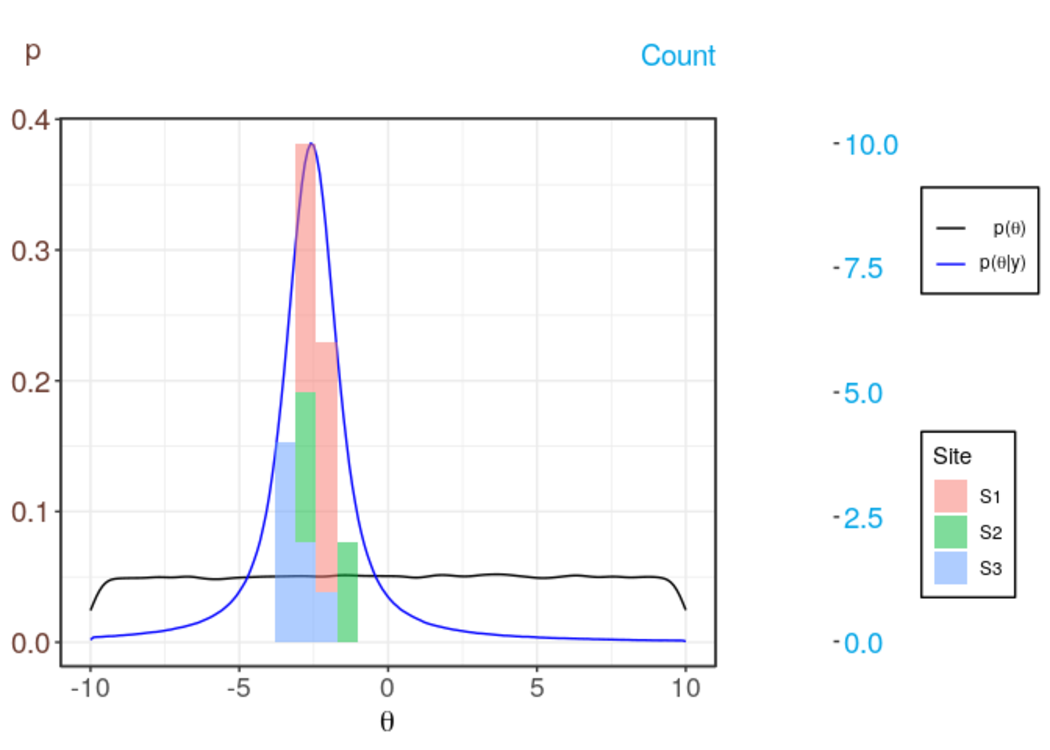
\includegraphics[width=0.475\textwidth]{img/no_spatial_correlation.pdf}
    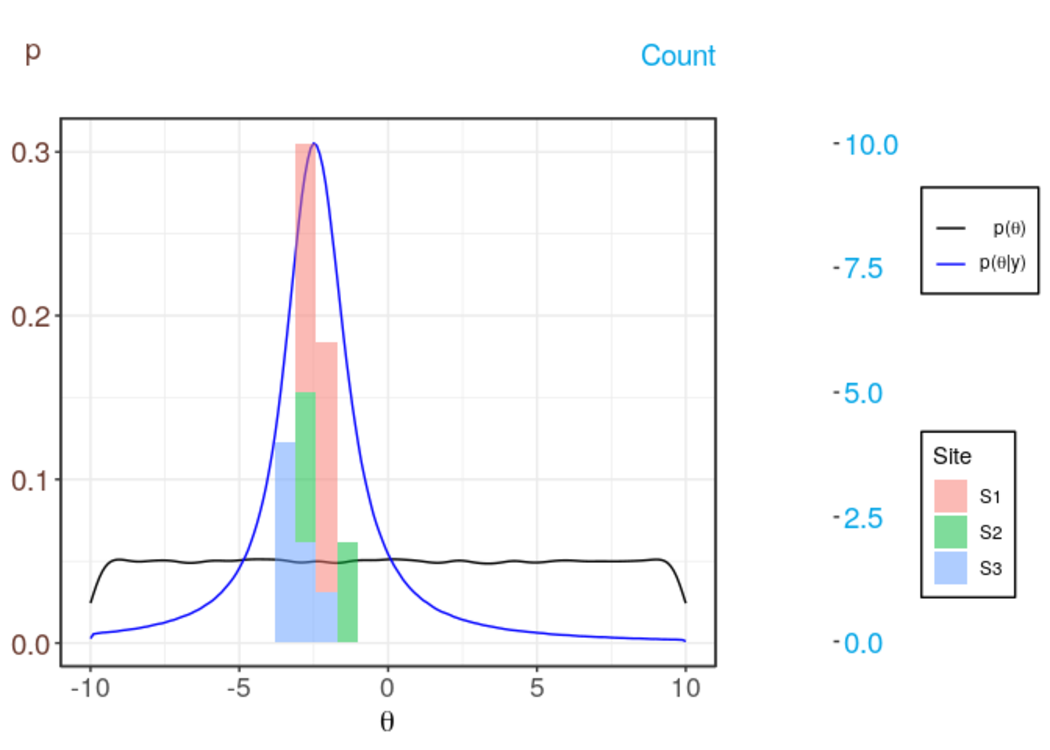
\includegraphics[width=0.475\textwidth]{img/spatial_correlation.pdf}
    \caption{Informative (blue) and non-informative (black) priors computed with \texttt{genExPrior()}. The left panel shows the prior without accounting for spatial correlation, whereas the right panel shows the prior accounting for spatial correlation (right panel). The colored bars represent the ex-situ data from the three different sites.}
    \label{fig:spatial_priors}
\end{figure}

To compare the effects of accounting for spatial correlation, we provide plots of the ex-situ prior with \texttt{spatialCoordinates} being both set to \texttt{FALSE} and \texttt{TRUE} (see the left and right panel in Figure \ref{fig:spatial_priors}, respectively). 
As can be seen, both priors look overall similar in shape. 
The main difference is that the latter shows a somewhat increased uncertainty, i.e., a wider variance, which can be seen by the increased mode of the distribution. 
The fact that the more realistic model produces more uncertain results may seem counterintuitive at first. 
However, the aim of statistical inference is not to reduce the uncertainty as much as possible but to correctly capture the uncertainty in the used data and the model.
As mentioned above, this problem of not accounting for possible correlations between measurements is called pseudoreplication and can have serious consequences by leading to overconfident statistical analyses.

\subsection{Example 4: Assimilating Multiple Data Types}\label{sec:multiple_data_types}

As mentioned above, \CRANpkg{exPrior} is written in a flexible manner, such that it can assimilate data that come in the form of measurements, bounds, or moments (see schematic in Figure \ref{fig:model_workflow}). 
To exemplify this flexibility, let us use in this example synthetic data from three sites labeled S1, S2, and S3. 
From Site S1, we have data in the form of bounds, where the minimum value of a hydrogeological property of S1 is 2, and its maximum value is 4. 
Site S2 has data in the form of moments, where the first moment, or site mean, is 2, while the second moment, or site variance, is 0.1. 
Finally, site S3 has three measurements.
Again, the associated vignette can be found at \url{https://github.com/GeoStat-Bayesian/exPrior/blob/master/vignettes/multi_type_data.Rmd}.
The code below shows how to format the data in \texttt{R} such that it can be read into \texttt{genExPrior()}.

\begin{example}
> exdata_S1 <- data.frame(val=c(2,4), site_id=rep('S1',2), 
+                         type=c('bound.min','bound.max'))
> exdata_S2 <- data.frame(val=c(2,0.1), site_id=rep('S2',2), 
+                         type=c('moment.1','moment.2'))
> exdata_S3 <- data.frame(val=c(2,3,4), site_id=rep('S3',3), 
+                         type=c('meas','meas','meas'))
> exdata <- rbind(exdata_S1, exdata_S2, exdata_S3)
\end{example}

As in previous examples, the data frame \texttt{exdata\_multitype} as well as the vector \texttt{theta} can be input directly into \texttt{genExPrior()} as such

\begin{example}
> resExPrior <- genExPrior(exdata = exdata, theta = seq(from=-10, to=10, by=0.1))
\end{example}

Finally, we can visualize the results \texttt{resExPrior} again using the \texttt{plotHyperDist} and \texttt{plotExPrior} functions.

\begin{example}
> plotHyperDist(resExPrior)
> plotExPrior(resExPrior)
\end{example}

\begin{figure}
    \centering
    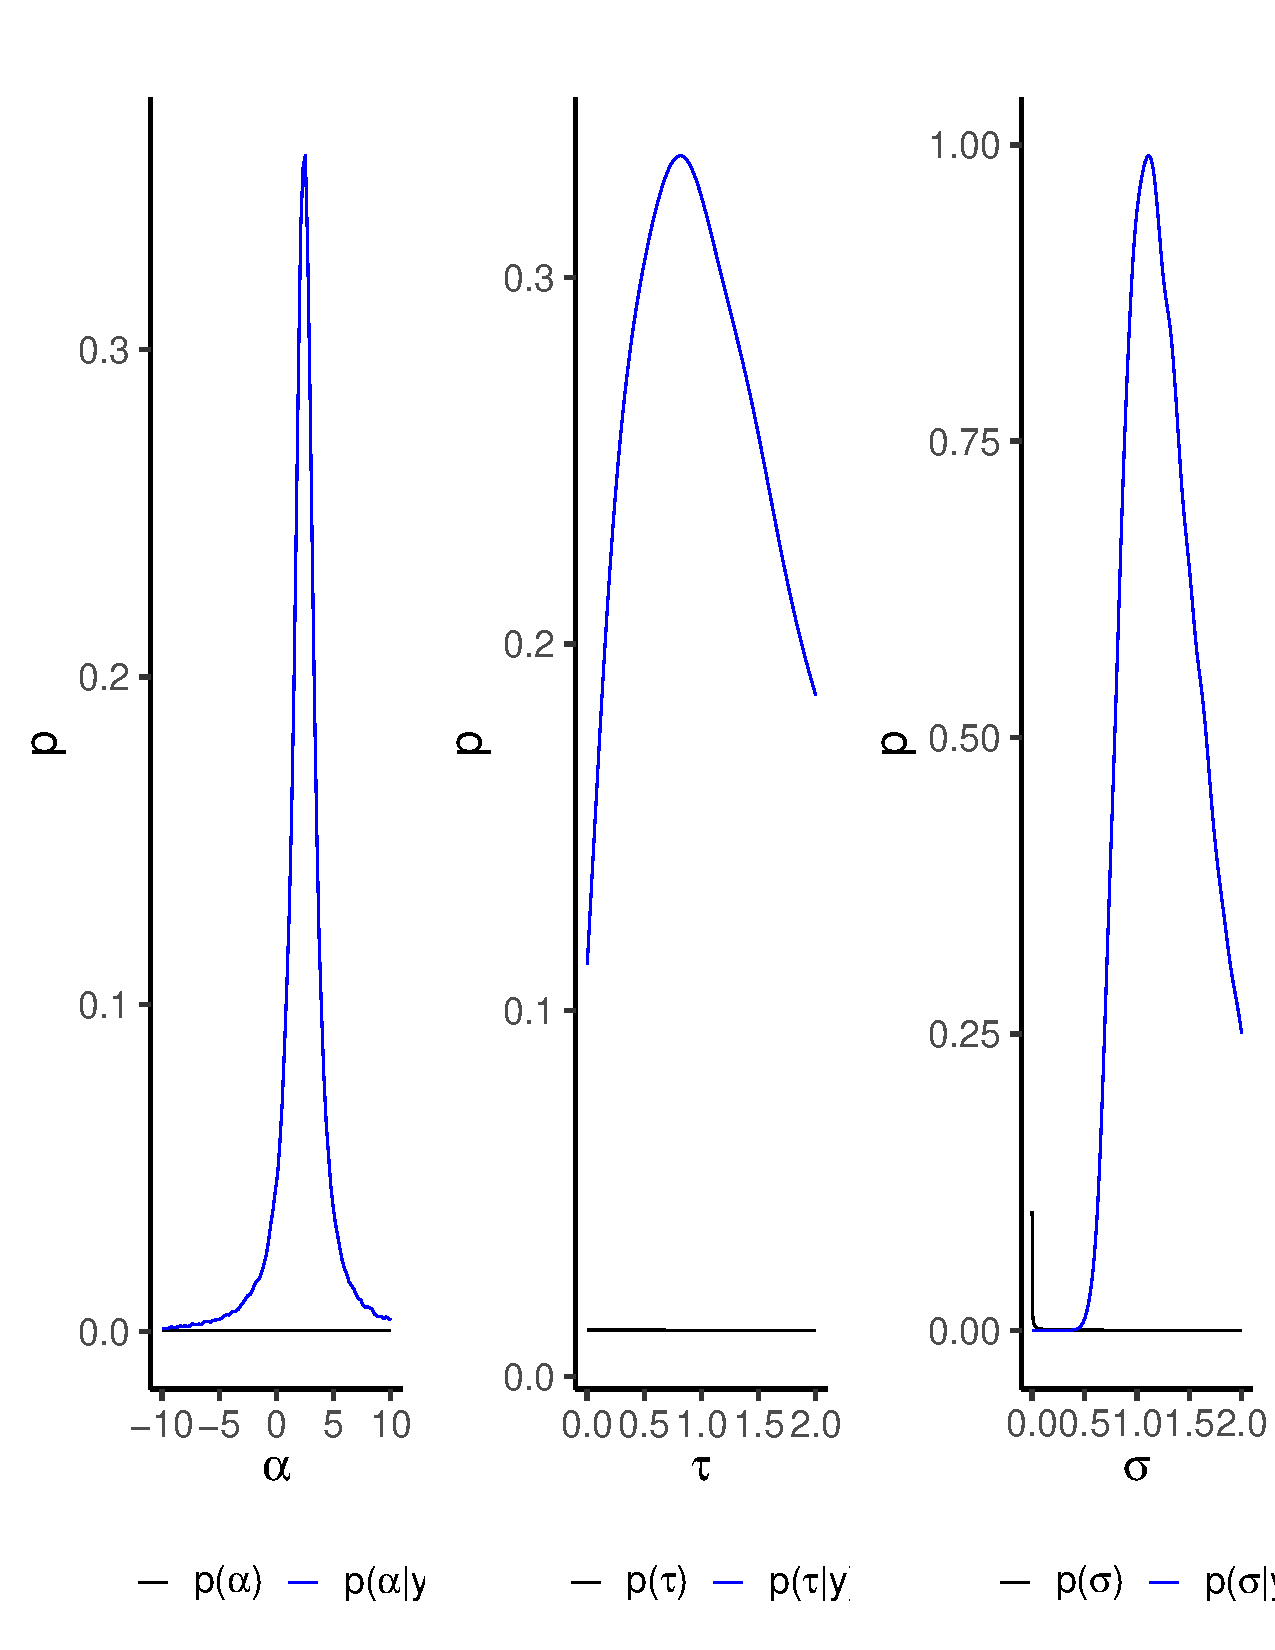
\includegraphics[width=0.45\textwidth]{img/example_4_hyperDist.pdf}
    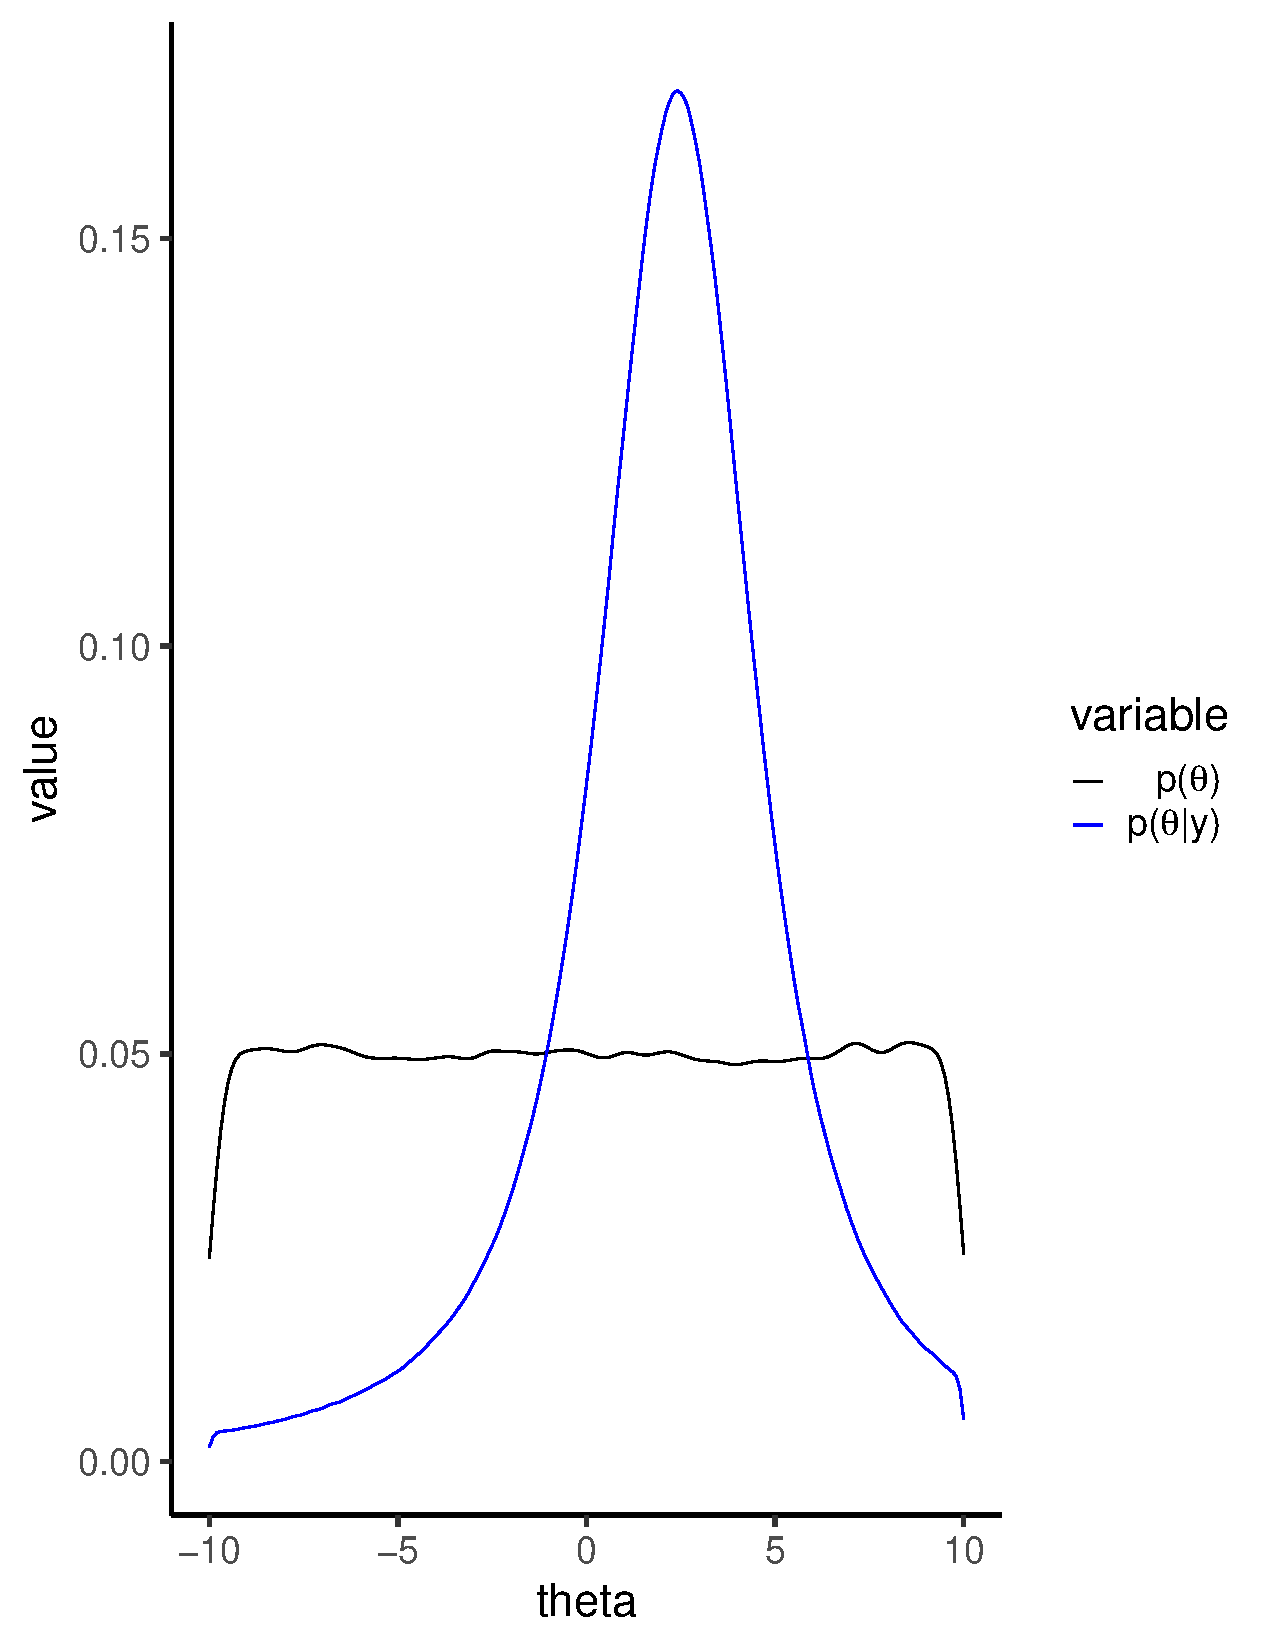
\includegraphics[width=0.45\textwidth]{img/example_4_exPrior.pdf}
    \caption{The left panel shows the distributions of the hyperparameters \texttt{alpha}, \texttt{tau}, and \texttt{sigma}. The right panel shows ex-situ data from three synthetic sites $S_1$, $S_2$, and $S_3$. The blue curve is the ex-situ prior computed using the data assimilation framework, while the black curve is the uninformative prior.}
    \label{fig:exdata_multiple_prior}
\end{figure}

The resulting hyperparameters and ex-situ prior distributions look very similar to the simple example from Section \ref{ssec:quick-example} (compare Figure \ref{fig:quick_example_prior} to Figure \ref{fig:exdata_multiple_prior}). 
This comparison shows that data in the form of bounds and moments can have a similar impact on the inference and how they can be assimilated by \texttt{exPrior}.


\section{Summary}

In this paper, we have introduced the \texttt{R} package \CRANpkg{exPrior}, which contains methods for assimilating ex-situ data to generate prior probabilities for geostatistical parameters. 
We explain the formulation of a prior distribution as a Bayesian Hierarchical Model (Section \ref{ssec:formulation}) and its implementation using \pkg{NIMBLE}, an \texttt{R} package created for efficient hierarchical modeling. 
We illustrate the model through a number of examples where \CRANpkg{exPrior} can be used, including univariate and multivariate models (Section \ref{sec:example-spatial}), as well as the assimilation of multiple data types (\ref{sec:multiple_data_types}). 
The package also contains data from the WWHYPDA, an open-source, hydrogeological database that provides valuable information for hydrogeological modeling. 
The goal of this package is to provide methods to facilitate geostatistical modeling, as well as to encourage the open-source and open-data movements between scientists.


\section{Acknowledgements}
This work has been partly funded by the German Research Foundation (DFG) under grant HE 7028/2-1, "What we talk about when we talk about uncertainty." 
Any opinions, findings and conclusions or recommendations expressed in this material are those of the authors and do not necessarily reflect the views of the DFG.


\bibliography{RJreferences}

\address{Falk He{\ss}e\\
  Institute of Earth and Environmental Sciences\\
  University Potsdam\\
  Potsdam, Germany\\}
  ORCiD: 0000-0002-2547-8102\\
\email{falk.hesse@ufz.de}

\address{Karina Cucchi\\
  Department of Civil and Environmental Engineering\\
  University of California, Berkeley\\
  Berkeley, CA, USA\\}
\email{karina.cucchi@berkeley.edu}

\address{Nura Kawa\\
  Department of Statistics\\
  University of California, Berkeley\\
  Berkeley, CA, USA\\
  currently at:\\
  Leuven Statistics Research Centre, \\
  KU Leuven, \\ 
  Leuven, Belgium\\}
\email{nkawa@berkeley.edu}

\address{Yoram Rubin\\
  Department of Civil and Environmental Engineering\\
  University of California, Berkeley\\
  Berkeley, CA, USA\\}
\email{rubin@ce.berkeley.edu}
